\documentclass[11pt,reqno]{amsart}
\usepackage{amsbsy,amsfonts,amsmath,amssymb,amscd,amsthm,mathrsfs}
\usepackage{subfigure,enumitem,graphicx,epsfig,color}
%\usepackage[colorlinks=true,citecolor=blue,linkcolor=red,urlcolor=blue]%{hyperref}
\usepackage[a4paper,left=3cm,right=3cm ,centering]{geometry}
%\usepackage[a4paper,centering,includefoot]%{geometry}

\renewcommand{\baselinestretch}{1.23}\normalsize
\usepackage{amsthm,dsfont,mathrsfs,amsmath,amssymb,amsfonts,euscript,mathtools}
\usepackage[pdfencoding=auto, psdextra]{hyperref}
%\usepackage{unicode-math}

\makeatletter
\let\oldHyPsd@CatcodeWarning\HyPsd@CatcodeWarning% Store original catcode warning
\renewcommand{\HyPsd@CatcodeWarning}[1]{% Update to check for...
  \ifnum\pdfstrcmp{#1}{math shift}=0    % ...the presence of 'math shift'. 
  
  \fi
}
\usepackage{graphicx}
\usepackage{authblk}
%\usepackage{blindtext}
%\makeatletter
\renewcommand\@author{\ifx\AB@affillist\AB@empty\AB@author\else
      \ifnum\value{affil}>\value{Maxaffil}\def\rlap##1{##1}%
    \AB@authlist\\[\affilsep]\behalf\\\AB@affillist
    \else  \AB@authors\fi\fi}
\makeatother
\usepackage{pict2e}
\usepackage{outlines}
\usepackage{enumitem}
%\usepackage[pagewise]\{lineno\}\linenumbers 
\usepackage{pxfonts}
\usepackage{srcltx}
%\usepackage[colorlinks=true,linkcolor=blue,citecolor=green]{hyperref}
%\usepackage[a4paper,text={6.1in,8in},centering,includefoot,foot=1in]{geometry}
\usepackage{tikz}
\renewcommand{\baselinestretch}{1.23}\normalsize
%\setlength{\parskip}{.05in} \setlength{\textheight}{22cm}
%\addtolength{\textheight}{\topskip}
\usepackage{parskip}
\theoremstyle{plain}
\newtheorem{mainthm}{Theorem}
\newtheorem{maincor}[mainthm]{Corollary}
\newtheorem{theorem}{Theorem}[section]
\newtheorem{lemma}[theorem]{Lemma}
\newtheorem{example}[theorem]{Example}
\newtheorem{conjecture}[theorem]{Conjecture}
\newtheorem{question}[theorem]{Question}
%\theoremstyle{definition}
\newtheorem{definition}[theorem]{Definition}
\newtheorem{corollary}[theorem]{Corollary}
\newtheorem{remark}[theorem]{Remark}
\newtheorem{assertion}[theorem]{Assertion}
\newtheorem{notations}[theorem]{Notations}
\newtheorem{proposition}[theorem]{Proposition}
\newtheorem{claim}[theorem]{Claim}
\newtheorem*{theorem A}{Theorem A}
\newtheorem*{theorem B}{Theorem B}
\newtheorem*{theorem C}{Theorem C}
\newtheorem*{theorem 1}{Theorem 1}
\newtheorem*{theorem 2}{Theorem 2}
\newtheorem*{theorem 3}{Theorem 3}
\renewcommand{\thesubfigure}{}
\renewcommand{\theenumi}{\roman{enumi}}
\renewcommand{\labelenumi}{\theenumi)}
\renewcommand{\theenumii}{\alph{enumii}}
\renewcommand{\labelenumii}{\theenumii)}
\renewcommand{\themainthm}{\Alph{mainthm}}
\renewcommand{\themaincor}{\Alph{mainthm}}
\newcommand{\eqdef}{\stackrel{\scriptscriptstyle\rm def}{=}}
\DeclareMathOperator{\IFS}{IFS}
\DeclareMathOperator{\diam}{diam}
\DeclareMathOperator{\vol}{vol}

\numberwithin{equation}{section}

\newcommand{\lmargin}[1]{{\marginpar{\tiny \textcolor{red}{L$\triangleright$ #1}}}}

\setcounter{tocdepth}{3}
\let\oldtocsection=\tocsection
\let\oldtocsubsection=\tocsubsection
\renewcommand{\tocsection}[2]{\hspace{0em}\bf\oldtocsection{#1}{#2}}
\renewcommand{\tocsubsection}[2]{\hspace{1em}\oldtocsubsection{#1}{#2}}
\let\oldtocsubsubsection=\tocsubsubsection
\renewcommand{\tocsubsubsection}[2]{\hspace{2em}\oldtocsubsubsection{#1}{#2}}
\usepackage{amsaddr}
%\makeatletter
%\renewcommand{\email}[2][]{%
%  \ifx\emails\@empty\relax\else{\g@addto@macro\emails{,%\space}}\fi%
  %\@ifnotempty{#1}%{\g@addto@macro\emails{\textrm{(#1)}\space}}%
%  \g@addto@macro\emails{#2}%
%}
%\makeatother
\usepackage{lipsum}
\title[Attracting invariant graphs and porcupine attractors]{Attracting invariant graphs and higher dimensional porcupine attractors}
\author[Zaj and Ghane]{M. Zaj  and F. H. Ghane}
\address[Zaj and Ghane]{Department Mathematics, Ferdowsi University of Mashhad}
%\affil[1]{Department of Computer Science, \LaTeX\ University}
%\affil[2]{Department of Mechanical Engineering, \LaTeX\ %University}
 \keywords{skew products, maximal attractor, synchronization, invariant graph, entropy.} \subjclass[2010]
{37A05; 37C40; 37C70; 37H15; 37D25; 37D30.}
\begin{document}


%\maketitle
%\maketitle
%%%%%%%%%%%%%%%%%%%%%%%%%%%%%%%%%%%%%%%%%%%%%%%%%%%%%
\begin{abstract}
We study discrete time skew product dynamical systems with higher dimensional fibers and
non-uniformly contracting fiber dynamics.
For an open class of such systems driven by expanding or solenoidal base maps, we establish a
sharp geometric-statistical dichotomy for maximal attractors: either the attractor is a
continuous invariant graph, or it is a \emph{solenoidal $n$-porcupine attractor} consisting of
a measurable invariant graph together with uncountably many embedded $C^{1}$ spines.

In the porcupine regime we identify a symbolic branching mechanism inside the blending region
that generates topological transitivity and positive topological entropy on the maximal
attractor.
This provides a rigorous source of chaotic dynamics without assuming uniform hyperbolicity or
the existence of Markov partitions.

To describe statistical behaviour under weak and non-uniform contraction, we introduce the
notion of \emph{fiberwise SRB-like measures}.
Under natural assumptions, these measures exist uniquely, are ergodic, and attract fiber
distributions at an exponential rate.
As a consequence, we obtain a robust form of \emph{statistical synchronization}, whereby
typical fiber distributions converge exponentially to a common invariant probability measure
despite the geometric complexity of the attractor.

Finally, we establish regularity criteria for invariant graphs, prove $C^{2}$ persistence and
parameter stability of the geometric and statistical dichotomy, and present a detailed example
verifying all hypotheses and illustrating the porcupine geometry, chaotic dynamics, and
statistical synchronization.
\end{abstract}

\maketitle
\thispagestyle{empty}
\tableofcontents



\section{Introduction}

Attractors in forced, random, or nonautonomous dynamical systems exhibit a wide range of
topological, geometric, and statistical behaviours depending on the perspective adopted,
including topological attractors, invariant graph attractors, pullback attractors, and
SRB--measure attractors
\cite{robinson1998dynamical,magal2005global}.
A unifying and flexible framework for studying such phenomena is provided by discrete time
skew products of the form
\begin{equation}\label{eq:skew}
F(\theta,y)=(S(\theta),f_\theta(y)),\qquad
F:\Theta\times Y\to\Theta\times Y,
\end{equation}
where $(\Theta,S)$ is a compact driving system and each map
$f_\theta:Y\to Y$ acts on a compact fiber space $Y$.
Skew products arise naturally in deterministic forcing, random and stochastic dynamics,
partially hyperbolic extensions, and time dependent control systems.
They capture the interaction between expansion or complexity in the base dynamics and
contraction, neutrality, or non-uniform behaviour in the fibers.
This interaction is responsible for many of the non-hyperbolic mechanisms observed in modern
applied and theoretical dynamics.


Skew products with weak or non-uniform contraction in the fiber direction arise broadly in
applications:

\begin{itemize}
\item \emph{Neuroscience and coupled oscillators.}
Forced neuron models and slow-fast synaptic systems often combine expanding phase dynamics
with multidimensional internal states subject to weak contraction.
Complex firing patterns and intermittent synchronization naturally correspond to nontrivial
fiber attractors.

\item \emph{Climate and geophysical models.}
Quasiperiodically or randomly driven energy--balance and climate models involve multidimensional
internal variables with non-uniform contraction.
Fiberwise statistical laws describe averaged climate responses, while synchronization reflects
alignment of internal climate modes.

\item \emph{Control systems and network dynamics.}
Hybrid controllers, symbolic switching protocols, and time dependent routing schemes often
exhibit expanding base actions coupled with weakly contractive internal subsystems.
Understanding long term behaviour under irregular forcing is essential for robustness and
stability.

\item \emph{Random dynamical systems and filtering.}
Nonlinear filtering and stochastic forcing frequently induce contraction of internal states,
leading to collapse of distributions toward invariant statistical laws.
A rigorous description of this convergence requires a fiberwise statistical framework.
\end{itemize}

These applications motivate the need for a unified theory of skew products with
higher dimensional fibers and non-uniform contraction, capable of describing both their
\emph{geometric structure} (graphs, multi graphs, porcupine type attractors) and their
\emph{statistical behaviour} (SRB-like measures and synchronization phenomena).

%\subsection*{Classical theory and limitations}

When the fiber dynamics is \emph{uniformly contracting}, classical results guarantee the
existence of a unique continuous invariant graph attracting all fibers; see Stark
\cite{stark1999regularity}.
In the case of one-dimensional fibers, finer geometric classifications have been obtained,
including pinched attractors, fat solenoids, and bony attractors
\cite{jager2003quasiperiodically,tsujii2001fat,kudryashov2010bony}.

From a statistical perspective, the foundational work of Alves--Bonatti--Viana
\cite{alves2000srb}
established the existence of SRB measures for partially hyperbolic systems whose central
direction is mostly expanding.
This theory explains how physical measures persist under strong non-uniformity, but it is
intrinsically expansion based and does not address statistical behaviour arising from
\emph{fiberwise contraction}.

Despite these advances, major challenges remain for forced systems and general skew products:

\begin{itemize}
\item most existing results either assume $\dim Y=1$ or rely on strong uniform hyperbolicity;
\item non-uniform contraction destroys classical graph regularity and produces geometric
structures, such as multi graphs and porcupines, with no one--dimensional analogue;
\item higher dimensional fibers lack the order and monotonicity tools available in dimension
one;
\item existing SRB theories do not describe statistical behaviour in weakly contracting fiber
regimes nor explain synchronization in this setting;
\item a unified geometric and statistical classification of maximal attractors for nonlinear skew
products has been lacking.
\end{itemize}

%\subsection*{Recent developments and remaining gaps}

Several recent works address parts of this picture, though none provides a complete
geometric statistical theory.

\medskip
\noindent\textbf{(A) Non-uniform geometry and multi--graphs.}
Rabiee--Ghane--Zaj~\cite{rabiee2022open} construct multi graph and bony multi graph attractors,
but only for one dimensional fibers and without statistical results or synchronization
phenomena.

\noindent\textbf{(B) Non-hyperbolic behaviour in dimension one.}
Barrientos--Cisneros~\cite{barrientos2024zero} and
Barrientos--Chávez~\cite{barrientos2024historical} demonstrate robust zero Lyapunov exponents
and historical behaviour in transitive skew products, again restricted to one dimensional
fibers.

\noindent\textbf{(C) Nonautonomous and fractional order systems.}
Cui--Kloeden~\cite{cui2024skew} establish existence of bounded skew product attractors for
fractional equations, but do not address nonlinear geometric classification or SRB type
statistics.

\noindent\textbf{(D) Invariant distributions and fractal graphs.}
Xu--Zhang~\cite{xu2024invariant} study invariant distributions and fractal graph structures,
without considering attractor classification or fiberwise statistics.

\noindent\textbf{(E) Empirical and variational approaches.}
Díaz et al.~\cite{diaz2022variational} and Crovisier et al.~\cite{crovisier2020empirical} provide
deep insights into ergodic measures and empirical distributions under weak hyperbolicity, but
not specifically for skew products with heterogeneous forcing.

\noindent\textbf{(F) SIAM-line advances in synchronization and linear theory.}
Recent SIAM contributions
\cite{jardon2024persistent,beyn2023angular,beyn2022angular}
develop synchronization criteria and angular-value theory for nonautonomous linear systems.
These tools do not address nonlinear geometric dichotomies or statistical synchronization in
skew products.

%\subsection*{Contributions of the present work}

This paper develops a unified geometric and statistical theory for skew products with
\begin{itemize}
\item fibers of dimension $\dim Y\ge2$,
\item non-uniform weak contraction in the fiber direction,
\item expanding or solenoidal base dynamics.
\end{itemize}

Our main contributions are as follows:

\begin{enumerate}[label=(\roman*)]

\item \textbf{Geometric dichotomy for maximal attractors.}
We prove a sharp dichotomy: for an open class of skew products, the maximal attractor is either
(a) a continuous invariant graph, or
(b) a \emph{solenoidal $n$--porcupine attractor} consisting of a measurable invariant graph
together with uncountably many embedded $C^1$ spines.
This provides the first such classification for higher dimensional, non-uniformly contracting
fibers.

\item \textbf{Chaotic dynamics inside porcupine attractors.}
In the porcupine regime we prove the existence of symbolic branching mechanisms that generate
topological transitivity and positive topological entropy on the maximal attractor.
This establishes the presence of chaotic dynamics without assuming uniform hyperbolicity or
Markov partitions.

\item \textbf{Fiberwise SRB-like measures.}
We introduce the notion of \emph{fiberwise SRB-like measures} describing statistical behaviour
inside weakly contracting fibers.
We prove existence, uniqueness, ergodicity, and exponential convergence, extending the SRB
program of \cite{alves2000srb} to contraction dominated skew products.

\item \textbf{Statistical synchronization.}
Despite the geometric complexity of porcupine attractors, fiber distributions converge
exponentially to the unique fiberwise SRB-like measure.
This phenomenon, which we term \emph{statistical synchronization}, has no analogue in
one dimensional geometric studies and no counterpart in expansion based SRB theory.

\item \textbf{Regularity, robustness, and examples.}
We establish regularity criteria for invariant graphs, analyze the breakdown of regularity
under loss of uniform contraction, prove $C^2$ persistence of the dichotomy, and provide a
detailed example verifying all hypotheses.
\end{enumerate}

%\subsection*{Organization of the paper}

%Section \ref{s2} develops tools for random iterations of weakly contractive maps.
%Section \ref{wbr} constructs blending regions and covering mechanisms.
%Section \ref{sec3} proves the geometric dichotomy.
%Section \ref{secchaotic} establishes chaotic dynamics in the porcupine regime.
%Sections \ref{Statistical} and \ref{secexample} develop symbolic separation and entropy estimates.
%Section~8 constructs fiberwise SRB-like measures and proves statistical synchronization.
%Section~9 presents a detailed example illustrating the theory.




%%%%%%%%%%%%%%%%%%%%%%%%%%%%%%%%%%%%%%%%%%%%%%%%%%%%%
\subsection{Attractors and Skew Products}
We start recalling some classical definitions related to attractors.
Many variants for the definition of an attractor can be found in the literature,
see \cite{milnor1985concept} for a discussion.
In what follows, let  $M$  be a compact, connected, closed, and smooth Riemannian manifold,  $m$ the normalized Lebesgue measure on $M$, and
 $\psi \colon M \to M$ a continuous map.

 Given a closed $\psi$-invariant set $A$,  its \emph{basin of attraction} $B(A)$ is the set of points   whose future orbits tend  (in the Hausdorff metric) to $A$.
  We say that $A$ is  \emph{Milnor attractor} for $\psi$
if $m(B(A))>0$ \cite{milnor1985concept}.
In some definitions of attractors, the basin of attraction $B(A)$ is an open set. However, here we only
require a basin of attraction with positive measure.

A compact set $D$ is called \emph{trapping} for $\psi$ if $\psi(D) \subset \textnormal{int}(D)$, where $\textnormal{int}(D)$ denotes the interior of $D$. In such a case,  the
closed $\psi$-invariant set
\begin{equation}\label{e18}
A_{max}(D,\psi):= \bigcap_{n\geq 0}\psi^n(D)
\end{equation}
is  the \emph{maximal attractor} for $\psi$ in $D$.

In discrete time, random dynamical systems influenced by a deterministic external factor are modeled as skew product systems. 
 Consider compact metric spaces $\Theta$ and $Y$ and a continuous map
$S \colon \Theta \to \Theta$. Fixed $S$, we denote by $\mathcal{C}_{S, \mathrm{Lip}} (\Theta\times Y)$ the set of skew products
\begin{equation}
%\label{e.asin}
F=F_{(S,f_{\theta})} \colon \Theta \times Y \to \Theta \times Y, \qquad
F(\theta,y) =(S(\theta), f_\theta(y)),
\end{equation}
whose fiber maps $f_\theta$, $\theta \in \Theta$, are Lipschitz and continuously depend on $\theta$. Here, $S$ denotes the {\em{base transformation}} 
 and $f_\theta$ represents the {\em{fiber transformation}} (or {\em{forced system}}). 

   The fiber map $f_\theta$ can be considered as a map
from $Y$ to $ Y$, where $ Y$ is the fiber space.
We adopt the usual notation $ F^{n}(\theta,y ) = (S^{n}\theta , f_{\theta}^{n}(y))$,
for the iterates $F^{n}$ of $F$, where $f^{n}_{\theta} = f_{S^{n-1}(\theta)} \circ \cdots \circ f_{\theta}$.
Hence, $f_\theta^{n+k}(y) = f_{S^k \theta}^n (f^k_\theta(y))$. If the fiber maps are invertible, for $n = 1$ and $k =-1$ this includes the identity and $f_\theta^{-1}(y) = (f_{S^{-1}\theta})^{-1}(y)$.
%%%%%%%%%%%%%%%%%%%%%%%%%%%%%%%%%%%%%%

\subsection{Invariant graphs}\label{assp}
We now discuss invariant graphs and their variations.
 In the study of skew products, invariant graphs, particularly attracting invariant graphs, play an essential role. In fact, they are the natural substitutes of fixed points and considerably simplify the dynamics of the forced systems.

\begin{definition}    
Let $m$ be a $S$-invariant measure. A measurable function $\gamma:\Theta \to Y$ is
\begin{enumerate}         
  \item[i)]
  an {\em{$F$-invariant graph}} if for every $\theta \in \Theta$ it holds
$$
F(\theta,\gamma(\theta))=(S(\theta),\gamma(S(\theta))), \quad \text{or} \quad f_\theta(\gamma(\theta))=\gamma(S(\theta)),
$$
  \item[ii)]
  an {\em{$(F,m)$-invariant graph}} if
\begin{equation}\label{1graph}
 f_\theta(\gamma(\theta))=\gamma(S(\theta)),  \quad \text{for} \ m-a.e. \ \theta\in \Theta.
\end{equation}
\end{enumerate}
\end{definition}

With slight abuse of notation, we call the point set
$$
\Gamma=\Gamma_\gamma :=\{(\theta,\gamma(\theta)):\theta \in \Theta\} 
$$
$F$ or $(F,m)$-invariant graph as well, but labeled with
the corresponding capital letter.

The graph $\Gamma$ is an attracting invariant graph if for $m$-a.e. $\theta \in \Theta$, one has that
\begin{equation*}
  \lim_{n \to \infty}|\pi_y(F^n(\theta,y))-\gamma(S^n(\theta))|=0,
\end{equation*}
for all $y \in Y$.

In skew products, Lyapunov exponents  are  useful quantitative indicators of the asymptotic expansion and contraction rates (along  fibers).
\begin{definition}[Maximal Lyapunov exponent]\label{max}
Let $F :\Theta \times Y \to \Theta \times Y$  be a skew product whose fiber maps $f_\theta$ are differentiable. The {\em{maximal Lyapunov exponent of an $F$-invariant probability measure $\mu$}} is defined by

\begin{equation}\label{lya1}
 \lambda(\mu,F):=\lim_{n \to \infty}\frac{1}{n}\int_{\Theta \times Y} \log \|Df_\theta^{n}(x)\| \, d\mu(\theta,x).
\end{equation}
The {\em{maximal Lyapunov exponent of an $(F ,m)$-invariant graph $\gamma$}} is defined by
\begin{equation}\label{lya}
 \lambda_m(\gamma):=\int_{\Theta} \log \|Df_\theta(\gamma(\theta))\|\,dm(\theta).
\end{equation}
\end{definition}

%%%%%%%%%%%%%%%%%%%%%%%%%%%%%%%%%%%%%%
%%%%%%%%%%%%%%%%%%%%%%%%%%%%%%%%%%%%%%%%%%%%
\subsection{Partial hyperbolicity}
Consider a smooth manifold $M$ (maybe noncompact), a differentiable dynamical system $f:M \to M$ and an $f$-invariant set $\Lambda$. A splitting $T_{\Lambda}M=E\oplus F$ is \emph{dominated} if $E$ and $F$ are $Df$-invariant and there are constants $m>0$ and $K< 1$ such that
\begin{equation}\label{dom}
  \|(D_xf^m) |_{E_x}\| \|((D_xf^m)^{-1}) |_{F_{f^m(x)}}\|<K, \ \text{for \ all} \ x\in \Lambda.
\end{equation}
A $Df$-invariant bundle $E$ defined on $\Lambda$ is uniformly contracting (resp. expanding) if there are $C>0$ and $0< \lambda<1$ such that for every $n>0$ one has
\begin{equation}\label{ce}
  \|D_xf^n(v)\| \leq C\lambda^n \|v\| \ \ (\text{resp.} \ \|D_xf^{-n}(v)\| \leq C\lambda^n \|v\|) \ \text{for \ all} \ x\in \Lambda \ \text{and} \ v \in E.
\end{equation}
We say that the set $\Lambda$ is \emph{partially hyperbolic} if there is a dominated splitting
$E\oplus F$ of $T_{\Lambda}M$ such that either $E$ is uniformly contracting or $F$ is uniformly expanding.
In the first case we write $T_{\Lambda}M=E^{ss}\oplus E^{cu}$, otherwise we write $T_{\Lambda}M=E^{uu}\oplus E^{cs}$.

An $f$-invariant set $\Lambda$ is \emph{strongly partially hyperbolic} if there is a $df$-invariant dominated splitting
$E^s \oplus E^c \oplus E^u$ where $df_{|E^s}$ is uniformly contracting, $df_{|E^u}$ is uniformly
expanding, $E^c$ is non-trivial and non-hyperbolic, and the three bundles $E^s$, $E^c$, and $E^u$ are non-trivial.

\subsection{Main results}\label{mm}
The space of all skew products $F_{(\ell, f_t)}$
as in \eqref{skewT1} is denoted by $\mathcal{C}_\ell(\mathbb{T}^1\times \mathbb{B}_n)$.
We denote by $\mathcal{C} (\mathcal{S}_\ell \times \mathbb{B}_n)$
the space of skew product maps $\mathbb{F}= \mathbb{F}_{F}$
which are an extension of some
$F\in \mathcal{C}_\ell(\mathbb{T}^1\times \mathbb{B}_n)$.
We equip these spaces with the metric given by \eqref{e113}

For the skew product with trapping region $D$, the set $\Lambda:=A_{max}(D)$ is the maximal attractor. 
Given any point $a$ in the base space let $\Lambda_a:=\Lambda \cap \{a\}\times \mathbb{B}_n$. We call $\Lambda_a$ a \emph{spine} and say that it is \emph{non-trivial} if it is not a singleton.
Note that for any $a$ in the base space, $\Lambda=\bigcup_{}\Lambda_a$.

%\begin{remark}\label{mfi}
%Note that the baker map $\Phi_\ell$ preserves Lebesgue measure, denoted by %$\nu_{\Phi_\ell}$, and is ergodic \cite{devaney1981baker}.
%\end{remark}
The following concept is a generalization of porcupine horseshoes discovered by Diaz and Gelfert in \cite{diaz2010porcupine}.
Now, we define Solenoidal porcupine-like graph as follows:

\begin{definition}[Solenoidal porcupine-like graph]\label{sol}
Given $\mathbb{F} \in \mathcal{C}(\mathcal{S}_\ell \times \mathbb{B}_n)$,
a compact $\mathbb{F}$-invariant set $\Lambda$ is
a {\em{solenoidal $n$-porcupine-like graph}} if
\begin{enumerate}
  \item [(1)] $\Lambda$ is the maximal attractor for $\mathbb{F}$ in some trapping region $D$;
  \item [(2)]   there exist a subset $\widetilde{\mathcal{S}}_\ell$ of $\mathcal{S}_\ell$ with
  $\nu_\ell(\widetilde{\mathcal{S}}_\ell)=1$
    and an $(\mathbb{F},\nu_\ell)$-invariant (attracting) graph $\gamma_{\mathbb{F}}$
    defined on   $\widetilde{\mathcal{S}}_\ell$
     such that
  $\Lambda$ is the union of  the graph $\Gamma_{\gamma_{\mathbb{F}}}$  and a set
  consisting
of uncountably many one dimensional $C^1$ closed submanifold
contained in the closure of $\Gamma_{\gamma_{\mathbb{F}}}$ (called {\em{nontrivial spines}}).
The map $\gamma_{\mathbb{F}}$ is called  the {\em{graph function of the maximal attractor.}}
  \end{enumerate}
  \end{definition}


\begin{figure}[ht]
\centering
\begin{tikzpicture}[scale=1.1]
% --- Left box: invariant graph ---
\draw[thick] (-4.8,-1.8) rectangle (-0.3,2);
\node at (-2.55,2.25) {\textbf{(A) Invariant Graph}};
% axes
\draw[->] (-4.5,-1.6) -- (-4.5,1.8);
\draw[->] (-4.6,-1.5) -- (-0.5,-1.5);
\node at (-4.7,1.6) ;
\node at (-2.5,-1.75);
% smooth invariant graph
\draw[ultra thick,blue!60]
(-4.5,-0.3) .. controls (-3.3,1.2) .. (-2.3,0.8)
           .. controls (-1.5,0.5) .. (-0.5,0.2);
% --- Right box: porcupine attractor ---
\draw[thick] (0.3,-1.8) rectangle (4.8,2);
\node at (2.55,2.25) {\textbf{(B) Porcupine Attractor}};
% axes
\draw[->] (0.6,-1.6) -- (0.6,1.8);
\draw[->] (0.5,-1.5) -- (4.5,-1.5);
\node at (0.4,1.6) ;
\node at (2.5,-1.75) ;
% measurable backbone graph
\draw[ultra thick,blue!60]
(0.6,-0.1) .. controls (1.6,0.4) .. (2.6,0.25)
          .. controls (3.4,0.1) .. (4.3,0.0);
% deterministic spines (no randomness)
\foreach \x/\h in {0.6/1.4,1.1/1.0,1.6/1.5,2.1/1.2,2.6/1.7,3.1/1.3,3.6/1.6,4.1/1.1} {
    \draw[red!70!black,thick] (\x,0.0) -- (\x,\h);
}
\end{tikzpicture}
\caption{
Schematic representation of the geometric dichotomy for maximal attractors in skew
products with non-uniformly contracting fibers.
In the absence of a continuous invariant graph, the maximal attractor exhibits a
\emph{solenoidal porcupine structure}, consisting of a measurable invariant graph
(the central core) decorated by uncountably many embedded $C^{1}$ spines.
Each spine arises from stable remnants of random fiber compositions and varies
measurably with the base point.
The figure illustrates how expansion in the base, combined with weak contraction
and parabolic behavior in the fibers, destroys global graph regularity while preserving
a compact attracting set, as described in Theorem \ref{thm1}.
}
\label{fig:dichotomy}
\end{figure}




Here we have three main results as follows:
\begin{enumerate}
\item [$\blacktriangleright$] Let $f$ be a $C^2$ weakly contractive injective map and $\mathcal{N}_f$ be a normally hyperbolic adapted $C^2$ neighborhood of $f$ as in Proposition \ref{open}.
Then for every sequence $\mathbf{t}=(\cdots, t_{-n}, \cdots, t_{-1}, t_0)$
  with values in $I$, such that for each $n$, $f_{t_{-n}} \in \mathcal{N}_f$ or $f_{t_{-n}}$ is a $C^2$ injective map with $f_{t_{-n}}(\mathbb{B}_n)\subset \text{int}(\mathbb{B}_n)$,
   the intersection
  \begin{equation*}
\Gamma_{\mathbf{t}}=    \bigcap_{k\ge 0}
    \mathbb{B}_{\mathbf{t}} (k),
    \qquad
    \mathbb{B}_{\mathbf{t}} (k) :=       f^k_{\mathbf{t}} (\mathbb{B}_{n})
      \end{equation*}
is either a single point or a one dimensional $C^1$ closed submanifold.


\item [$\blacktriangleright$] There is an open neighbourhood
 $ \mathcal{V}_{\mathcal{S}_\ell}$ in
 $\mathcal{C}(\mathcal{S}_\ell \times \mathbb{B}_n)$
such that every $\mathbb{F}\in \mathcal{V}_{\mathcal{S}_\ell}$ has a maximal attractor $A_{max}(\mathbb{F})$ that
is  topologically transitive and satisfies the following dichotomy:
 \begin{enumerate}
   \item [$-$] either $A_{max}(\mathbb{F})$ is an attracting continuous invariant graph;
   \item [$-$] or $A_{max}(\mathbb{F})$ is a solenoidal $n$-porcupine-like graph.
      \end{enumerate}

%%%%%%%%%%%%%%%%%%%%%%%%%%%%%%%%%%%%%%
%Note that the baker map $\Phi_\ell$ preserves Lebesgue measure denoted by $\nu_{\Phi_\ell}$ (see Remark \ref{mfi}).
%Assume $G \in \mathcal{B}_{\Phi_\ell}(\mathbb{T}^2 \times \mathbb{B}_n)$. We denote by $\mathcal{M}_{\nu_{\Phi_\ell}}(G)$
 %the space of all $G$-invariant probability measures $\mu_{\Phi_\ell}$ on $\mathbb{T}^2 \times \mathbb{B}_n$
%with marginal $\nu_{\Phi_\ell}$, that is the set of all $G$-invariant measures which project to $\nu_{\Phi_\ell}$ in the first coordinate.
\item [$\blacktriangleright$] For a weakly attracting pair $(f_1,\ldots,f_k)$  (as defined in definition \ref{weakpair}) with blending 
region $B$, and that the base map $T\colon M\to M$ preserves an ergodic
absolutely continuous probability $\nu$,  the skew product
$F(a,y)=(T(a),f_a(y))$ admits a fiberwise SRB-like measure. In addition this fiberwise SRB-like measure is unique and ergodic.
\end{enumerate}


%\begin{theorem 1}\label{t1}
%There are $\ell\in \mathbb{N}$ and an open set $\mathcal{V}=\mathcal{V}_{\ell, \mathbb{T}^2}$
%in $\mathcal{B}_{\Phi_\ell}(\mathbb{T}^2 \times \mathbb{B}_n)$
%such that for every $G$ in $\mathcal{V}$ the maximal attractor $A_{max}(G):=A_{max}(\mathbb{T}^2 \times \mathbb{B}_n)$  is either a continuous attracting invariant graph or a thick $n$-porcupine attractor. In particular, the set of skew products $G \in \mathcal{V}$ posses $n$-porcupine attractor is nonempty. 
%\end{theorem 1}
%%%%%%%%%%%%%%%%%%%%%%%%%%%%%%%%%%%%%%%%%
\subsection{Main ingredients and organization}
We will provide an overview of the paper's contents and briefly outline the main ideas used to prove the theorem. In Section \ref{wbr}, we introduce two local tools, namely the weakly attracting pair and the weakly blending region of $\mathbb{R}^n$, which allow us to construct $n$-porcupine attractors. To construct the weakly blending regions of $\mathbb{R}^n$, we consider contractive maps with non-uniform contraction rates, also known as weakly contractive maps. For a specific class of weakly contractive maps, the approach presented in \cite{alves2000srb} yields a bounded distortion property for random compositions of fiber maps.
Partial hyperbolicity is a crucial element in our approach. Furthermore, we demonstrate that under small perturbations of a weakly contractive map, the forward random iterations of the ball $\mathbb{B}_n \subset \mathbb{R}^n$ are either a single point or a $C^1$-submanifold (as shown in Proposition \ref{open}). Based on these findings, we investigate the existence of a weakly blending region for each compact ball $\mathbb{B}_n \subset \mathbb{R}^n$, as detailed in Theorem \ref{problend}.
Section \ref{s.attractinggraphs} is dedicated to studying skew products that have non-uniform contraction rates along the fibers. This particular condition enables us to utilize
\cite[Thm. 1.4]{stark1999regularity} to establish attracting invariant graphs. In Section \ref{sec3}, we complete the proof of Theorem 1 and introduce an open set $\mathcal{V}$ that meets the requirements outlined in Theorem 1. The maps within $\mathcal{V}$ have average fiber contraction rates, and their fiber maps exhibit a weakly blending region.
These are the primary ingredients involved in constructing $n$-porcupine attractors. 

%%%%%%%%%%%%%%%%%%%%%%%%%%%%%%%%%%%%%%%%%%%

\section{Random iterations of maps}\label{s2}

In this section, we consider contractive maps with non-uniform contraction rates.
Following \cite{alber1997principle}, given a metric space $(X,d)$ we say that a continuous map $f\colon X \to X$ is \emph{weakly contractive} if $d(f(x),f(y)) < d(x,y)$ for every $x,y \in X$ with $x\neq y$.
It is well-known, see \cite[Coro.~3]{jager2003quasiperiodically} and \cite{bielecki1995iterated}, that if $f$ is weakly contractive and $(X,d)$ is compact then $f$ has a unique fixed point $x \in X$ which is attracting in the sense that $\lim_{k \to \infty}f^k(y)=x$, for every $y \in X$.
Here, we take $X=\mathbb{B}_n$, where $\mathbb{B}_n$ denotes the closed unit ball of $\mathbb{R}^n$.
Thus, for a weakly contractive map $f \colon \mathbb{B}_n \to \mathbb{B}_n$, we can speak of its \emph{attracting fixed point}, denoted by $x_f$.

A key ingredient in our construction of weak blending regions is the following:

\begin{definition}[Parabolic attracting fixed point]
Let $f\colon \mathbb{B}_n \to \mathbb{B}_n$ be a smooth weakly contractive map.
The attracting fixed point $x_f$ of $f$ is \emph{parabolic} if the Jacobian matrix $Df(x_f)$ possesses $1$ as a simple eigenvalue and the other eigenvalues have absolute values less than $1$.
The parabolic fixed point $x_f$ is \emph{generic} whenever the eigenvalues of $Df(x_f)$ are all positive and of multiplicity one.
\end{definition}

In what follows, we denote by $\mathbb{WC}^2 ( \mathbb{B}_n)$ the set of $C^2$ weakly contractive injective maps $f\colon \mathbb{B}_n \to \mathbb{B}_n$ with $f(\mathbb{B}_n)\subset \text{int}(\mathbb{B}_n)$ and whose attracting fixed point $x_f$ is generic and parabolic.
Note that $x_f$ belongs to the interior $\text{int}(\mathbb{B}_n)$ of $\mathbb{B}_n$.
There is a basis of neighborhoods $V_{n,f}$ of $x_f$ with $f(\overline{V_{n,f}}) \subset V_{n,f}$.
We call these neighborhoods \emph{attracting}.

\subsection{Bounded distortion property for weakly contractive maps}

Following the approach in \cite{alves2000srb, zaj2018physical}, for maps $f\in \mathbb{WC}^2 ( \mathbb{B}_n)$, we will provide a bounded distortion property on a region around its attracting fixed point $x_f$.
We start with some preparatory results.

\subsubsection{Dominated splittings, cone fields, and the strong stable foliation}

Given $f\in \mathbb{WC}^2 ( \mathbb{B}_n)$, consider the $Df$-invariant splitting $E^{ss} \oplus E^{c}$, corresponding to the eigenspaces of $Df(x_f)$ associated to the eigenvalues less than $1$ and equal to $1$, respectively.
Note that $E^c$ is one-dimensional.
As this splitting is dominated, we can extend it to a continuous splitting (also denoted by $E^{ss}\oplus E^{c}$) defined on a small attracting neighborhood $V_f$ of $x_f$.
Note that this new splitting is not necessarily invariant.

For notational convenience, we will use the adapted metric (equivalent to the initial one) provided by \cite[Theorem 1]{gourmelon2007adapted}.
This allows us to take the constant $C$ in equation \eqref{ce} equal to $1$.
Hence, there exists $0< \lambda<1$ such that
\begin{enumerate}
\item $\|D f|_{E^{ss}_x}\| \leq \lambda$, for all $x \in \overline{V_f}$;
\item $\|D f|_{E^{ss}_x}\| \cdot \|D f^{-1}|_{E^{c}_{f(x)}}\| \leq \lambda<1$ for all $x \in \overline{V_f}$.
\end{enumerate}
Recalling that $x_f$ is parabolic, by shrinking $V_f$ and slightly increasing $\lambda<1$ if necessary, we have the following strong form of domination
\begin{equation}
\label{strongversionii}
\|D f|_{E^{ss}_x}\| \leq \lambda \quad \text{and} \quad \|D f|_{E^{ss}_x}\| \cdot \|D f^{-1}|_{E^{c}_{f(x)}}\|^{1+1} \leq \lambda< 1,
\end{equation}
for all $x \in \overline{V_f}$.

For each $0<\beta<1$, we define the \emph{center cone field} $\mathcal{C}_\beta ^{c}:= (\mathcal{C}_\beta ^{c}(y))_{y \in \overline{V_f}}$ of width $\beta$ by
\begin{equation*}
\mathcal{C}_\beta ^{c}(y):=\{v_1 +v_2 \in E^{ss}_y \oplus E^{c}_y : \|v_1\| \leq \beta \|v_2\|\}.
\end{equation*}
The strong stable cone field $\mathcal{C}_\beta ^{ss}:= (\mathcal{C}_\beta ^{ss}(y))_{y \in V_f}$ of width $\beta$ is analogously defined.

The center cone field is positively invariant, that is $Df(y)( \mathcal{C}_\beta ^{c}(y)) \subset \mathcal{C}_\beta ^{c}(f(y))$, provided that $V_f$ is small and $y, f(y)\in \overline{V_f}$.
Indeed, according to (ii) above,
$$
Df(x_f)(\mathcal{C}_\beta ^{c}(x_f)) \subset \mathcal{C}_{\lambda \beta} ^{c}(x_f) \subset \mathcal{C}_\beta ^{c}(x_f).
$$
By continuity, this extends (for small $V_f$) to each $y \in \overline{V_f} \cap f^{-1}(\overline{V_f})$.

By \cite{brin1974partially, hirsch1977invariant}, the domination property and the uniform contraction of $E^{ss}$ imply that there is a (uniquely defined) continuous family $\mathcal{F}^{ss}$ of injectively $C^2$ immersed submanifolds $\{\mathcal{F}^{ss}(x) \colon x \in V_f \}$ of dimension $(n-1)$ such that $x \in \mathcal{F}^{ss}(x)$ and $\mathcal{F}^{ss}(x)$ is tangent to $E^{ss}_x$ at $x$.
This family is invariant, in the sense that $f(\mathcal{F}^{ss}(x))\subset\mathcal{F}^{ss}(f(x))$ for every $x \in V_f \cap f^{-1}(V_f)$, and the leaves $\mathcal{F}^{ss}(x)$ are uniformly contracted by $f$.
The lamination $\mathcal{F}^{ss}$ is called \emph{strong stable foliation} and the sets $\mathcal{F}^{ss}(x)$ are called \emph{strong stable leaves}.

Since the central bundle $E^{c}$ is one-dimensional, there always exist curves tangent to $E^c$ passing through every point in $V_f$.
These curves are called \emph{central leaves} and denoted by $\mathcal{F}^{c}(x)$.
In general, these central curves are neither invariant nor uniquely defined.
We now focus on these central curves and their iterations.

\subsubsection{Curves tangent to the central cone field and their iterations}\label{sss.curvestangento}

The next remark is a standard consequence of the persistence of domination and invariant bundles, see for instance \cite[Section B1]{bonatti2004dynamics}.

\begin{remark}\label{pert}
Consider $f\in\mathbb{WC}^2 ( \mathbb{B}_n)$, its attracting parabolic fixed point $x_f$, and a small attracting neighbourhood $V_f$ of $x_f$.
After increasing $\lambda <1$ and shrinking $V_f$, we can assume that the dominated splitting $E^{ss} \oplus E^{c}$ is defined on $\overline{V_f}$ and satisfies \eqref{strongversionii} and there is small $\beta>0$ such that
\begin{equation}\label{e3}
\|Df(y)v^{ss}\| \cdot \|Df^{-1}(f(y))v^{c}\| \leq \lambda \|v^{ss}\| \cdot \|v^{c}\|,
\end{equation}
for every pair of vectors $v^{ss}\in \mathcal{C}^{ss}_\beta(y)$, $v^c \in \mathcal{C}^c_\beta(y)$ and every point $y \in \overline{V_f} \cap f^{-1}(\overline{V_f})$.
Moreover, we can assume that there exists a $C^2$-neighborhood $\mathcal{N}_f$ of $f$ consisting of maps $g$ such that $g(\overline V_f) \subset V_f$, the domination conditions in \eqref{strongversionii} hold, $\|D g|_{E^{ss}_x}\| \leq \lambda$, the central cone field is $Dg$-invariant, i.e., $Dg(y)\mathcal{C}^c_\beta(y)\subset \mathcal{C}^c_\beta(g(y))$, and
\begin{equation}\label{e4}
\|Dg(y)v^{ss}\| \cdot \|Dg^{-1}(g(y))v^{c}\| \leq \lambda \|v^{ss}\| \cdot \|v^{c}\|,
\end{equation}
for every $v^{ss} \in \mathcal{C}_\beta ^{ss}(y)$, $v^{c} \in \mathcal{C}_\beta ^{c}(y)$, and every $y \in \overline{V_f} \cap g^{-1}(\overline{V_f})$.

As a consequence, the maximal invariant set of $g$ in $\overline{V_f}$ is partially hyperbolic with one dimensional central bundle and $(n-1)$-strong stable direction.
\end{remark}

In what follows, we fix $f\in\mathbb{WC}^2 ( \mathbb{B}_n)$, neighbourhoods $V_f$ of $x_f$ and $\mathcal{N}_f$ of $f$, and cone fields $\mathcal{C}_\beta ^{ss}$ and $\mathcal{C}_\beta ^{c}$ satisfying Remark~\ref{pert}.

A closed $C^1$-curve $N\subset V_f$ is \emph{tangent to the central cone field $\mathcal{C}_\beta ^{c}$} if for every $x\in N$ the tangent space $T_xN$ is contained in $\mathcal{C}_\beta ^{c}$.
We call these curves \emph{central} ones.
A special case of central curves are the central leaves.
Given a central curve $N$, the invariance conditions in Remark~\ref{pert} imply that for every $g \in \mathcal{N}_f$ we have that $g(N) \subset V_f$ and $g(N)$ is tangent to $\mathcal{C}_\beta ^{c}$.
Inductively, we have that if $g_1, \dots, g_n \in \mathcal{N}_f$ then $g_n \circ \cdots \circ g_1 (N) \subset V_f$ and the curve $g_n \circ \cdots \circ g_1 (N) $ is a central curve.

Similarly, we define $(n-1)$ disks tangent to the strong stable cone field and call them \emph{strong stable} disks.
Applying Remark~\ref{pert}, we have that if $g \in \mathcal{N}_f$ and $D$ is a strong stable disk such that $D\subset V_f$ and $g^{-1}(D) \subset V_f$ then $g^{-1}(D)$ is a strong stable disk with $\diam (D) \le \lambda \diam (g^{-1} (D))$.
Inductively, if $g_1, \dots, g_n \in \mathcal{N}_f$ and $D\subset V_f$ is a strong stable disk such that $g_i^{-1} \circ \cdots \circ g_1^{-1} (D) \subset V_f$ for every $i=1, \dots, n$, then $g_i^{-n} \circ \cdots \circ g_1^{-1} (D)$ is a strong stable disk such that
\begin{equation}
\label{e.stablecompositions}
\diam (D) \le \lambda^n \diam (g_i^{-n} \circ \cdots \circ g_1^{-1} (D)).
\end{equation}
Finally, given a set $A$ and a point $x\in A$, we denote by $C(x,A)$ the connected component of $A$ containing $x$.
We will consider the family of strong stable disks $\mathcal{F}^{ss}_{\mathrm{loc}}(x):= C(x,\mathcal{F}^{ss} (x)\cap V_f)$.

\subsubsection{Random iterations of central curves}
\label{sss.iterationsofcentralcurves}

In this subsection, we closely follow the constructions in \cite[Section 2.1]{alves2000srb} and omit some details.
Given a central curve $N$ as above, $x\in N$, and $\epsilon>0$, let $U_x (\epsilon)$ be the open $\epsilon$-neighborhood of $x$ in $\mathbb{B}_n$ and $N_x(\epsilon) := U_x(\epsilon) \cap N$.
There is small $r>0$ such that for each $x\in N$ there is a uniquely defined family of linear maps
$$
\mathcal{A}_x(y) \colon T_x N_x \to E_x^{ss}, \quad y \in N_x(r),
$$
such that the tangent spaces $T_y N_x$ are parallel to the graphs of $\mathcal{A}_x(y)$.

For given constants $C> 0$ and $0< \zeta \leq 1$, we say that the tangent bundle of $N$ is $(C, \zeta)$-\emph{H\"{o}lder} if there is $r>0$ such that
\begin{equation}\label{L}
\|\mathcal{A}_x(y)\| \leq C \rho(x, y)^{\zeta} \quad \textnormal{for every $x\in N$ and $y \in N_x (r)$},
\end{equation}
where $\rho(x, y)$ is the length of the curve connecting $x$ to $y$ in $N_x(r)$.
For $0< \zeta \leq 1$ we let
\begin{equation}
\label{e.curvaturek}
\kappa_\zeta(N):=\inf \{C > 0: \text{the tangent bundle of $N$ is $(C, \zeta)$-H\"{o}lder}\}.
\end{equation}

In \cite{alves2000srb} a H\"older exponent $\zeta$ is selected satisfying
$$
\|D f|_{E^{ss}_x}\| \cdot (\|D f^{-1}|_{E^{c}_{f(x)}}\|)^{1+\zeta} \leq \lambda<1.
$$
By equation \eqref{strongversionii}, we can take $\zeta=1$ and write $\kappa_1(N)= \kappa(N)$.
Next proposition is just a reformulation of \cite[Corollary 2.4]{alves2000srb} in our context of random compositions.
For that let us introduce some notation: given a sequence $\mathbf{t}=(\cdots, t_{-j}, \cdots, t_{-1}, t_0)$ and maps $f_{t_{-i}}\colon \mathbb{B}_n \to \mathbb{B}_n$, for each $j\ge 0$ we write
\begin{equation}
\label{e.compositionsoffs}
f^{j+1}_\mathbf{t} := f_{t_0}\circ f_{t_{-1}}\circ \cdots \circ f_{t_{-j}}.
\end{equation}
\begin{proposition}[Corollary 2.4 in \cite{alves2000srb}]\label{proj}
Let $f\in\mathbb{WC}^2 ( \mathbb{B}_n)$.
There are small neighborhoods $V_f$ of $x_f$ and $\mathcal{N}_f$ of $f$, a constant $\beta >0$ satisfying Remark~\ref{pert}, and a constant $C_1 > 0$ such that for every $C^1$-curve $N \subset V_f$ tangent to the centre cone field $\mathcal{C}_\beta ^{c}$, every continuous path $t \in I \mapsto f_t \in \mathcal{N}_f$, with $I \subset \mathbb{R}$ an interval, and every sequence $\mathbf{t}=(\cdots, t_{-j}, \cdots, t_{-1}, t_0)$ with values in $I$ the following holds:
\begin{enumerate}
\item [$a$)] there exists $n_0 \geq 0$ such that $\kappa(f_{\mathbf{t}}^{n}(N)) \leq C_1$ for every $n \geq n_0$,
\item [$b$)] if $\kappa(N)\leq C_1$ then the same is true for every $\kappa(f_{\mathbf{t}}^{n}(N))$, $n \geq 0$,
\item [$c$)] in particular, if $N$ is as in b), then the Jacobian functions
\begin{equation*}
J^n_{\mathbf{t},N} \colon f_{\mathbf{t}}^n(N) \ni y \mapsto \log |\det(D f |_{T_y f_{\mathbf{t}}^n(N)})|, \quad n \geq 0,
\end{equation*}
are $(L,1)$-H\"{o}lder continuous, for some $L > 0$ depending only on $C_1$ and $f$.
\end{enumerate}
\end{proposition}
A special case of Proposition~\ref{proj} is the non-random case where $f_{t_{-i}}=g\in \mathcal{N}_f$ for every $i$.

\subsubsection{Cusp-like regions}\label{cr}

Consider $f\in\mathbb{WC}^2 ( \mathbb{B}_n)$, a center leaf $\mathcal{F}^{c}(x_f)$ passing throughout $x_f$, and a closed fundamental domain $D^c$ of $\mathcal{F}^{c}(x_f)$ with boundary points $a\in V_f$ and $f(a)$.
For each $x\in D^c$ consider a small closed strong stable disk $D^{ss}(x)\subset \mathcal{F}^{ss}(x)$ containing the point $x$ in its interior and contained in $V_f$.
We choose these disks depending continuously on $x$ and such that $D^{ss}(f(a)):=f(D^{ss}(a))$.

Denote by $C^2(D^c, V_f)$ the space of $C^2$ maps from $D^c$ to $V_f$.
Let $H\colon D^{ss}(a) \to C^2(D^c, V_f)$ be a continuous map which associates to each $x \in D^{ss}(a)$ a $C^2$ arc $I_x:=H(x)(D^c)$ connecting the points $x$ and $f(x)$ such that $H(a)$ is the identity and hence $I_a=D^c$.
Thus, by shrinking the disks $D^{ss}(x)$, if necessary, we can assume that the curve $I_x$ is a central curve for every $x \in D^{ss}(a)$.
Consider now the closed subset
\begin{equation}\label{w1}
W_1:= \bigcup_{x \in D^{ss}(a)}I_x \subset V_f
\end{equation}
foliated by central curves and whose boundary contains the disks $D^{ss}(a)$ and $D^{ss}(f(a))$, see Figure~\ref{fig:cuspregion}.

By construction, the subsets $W_1$ and $f(W_1)$ are $C^2$ submanifolds contained in $V_f$.
Arguing recursively, we define the \emph{cusp-like region} $W$ as follows:
\begin{equation}\label{r02}
W:=\bigcup_{k=1}^\infty W_k, \quad \textnormal{where } W_k:=f(W_{k-1}),\quad k\ge 2.
\end{equation}

\begin{figure}[!ht]
\begin{center}
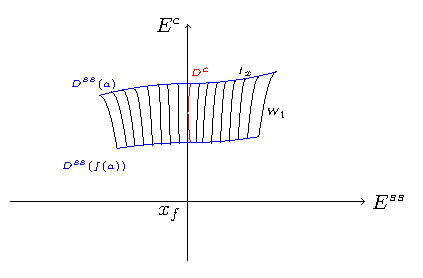
\includegraphics[scale=1.3]{blend-fig.pdf}
\caption{\small{The closed rectangle $W_1$.}}\label{fig:cuspregion}
\end{center}
\end{figure}

\begin{remark}\label{r2}{\em{
Note that $\diam(W_k)$ tends to zero as $k \to \infty$ and that the parabolic point $x_f$ satisfies $x_f \in \overline{W} \setminus W$.
Finally, the subsets $W_k$ and $W$ are $C^2$ submanifolds.}}
\end{remark}

Taking $f_{t_{-i}}=f$ for all $i$ in Proposition \ref{proj}, we have that the tangent bundle of the iterates $f^n(I_x)$ are H\"{o}lder continuous with uniform H\"older constants depending only on $f$ and $\kappa_1(D^c)$, see \eqref{e.curvaturek}.
Moreover, by continuity of $H$ and compactness of $I_x$ and $D^{ss}(a)$, we have that $\kappa_1(I_x)$ is uniformly bounded independently of $x$.
In particular, by item (c) of Proposition \ref{proj},
\begin{equation}\label{ten}
J^k_{I_x} \colon f^k(I_x) \ni y \mapsto \log |\det(Df|_{T_yf^k(I_x)})|
\end{equation}
is $(L, 1)$-H\"{o}lder continuous, for some constant $L > 0$ that does not depend on $k$ and $x$.

The observations above are summarized in the next proposition, which is a counterpart of \cite[Thm.~2.7]{zaj2018physical} in the $n$-dimensional case.

\begin{proposition}\label{thmcusp}
Let $f\in\mathbb{WC}^2 ( \mathbb{B}_n)$ and consider sufficiently small cusp-like region $W$ defined as in \eqref{r02}.
Then the function
\begin{equation*}
J : W \ni y \mapsto \log |\det(Df|_{T_y(W)})|
\end{equation*}
is $(L,1)$-H\"{o}lder continuous, for some constant $L > 0$.
\end{proposition}

\subsubsection{Random limits of a ball }\label{sss.randomlimits}

In this section, we prove the following result about forward random iterations of the ball $\mathbb{B}_n$.

\begin{proposition}\label{open}
Let $f\in\mathbb{WC}^2 ( \mathbb{B}_n)$.
There is a $C^2$ neighborhood $\mathcal{N}_f$ of $f$ such that for every continuous path $t \in I \mapsto f_t \in \mathcal{N}_f$ and every sequence $\mathbf{t}=(\cdots, t_{-n}, \cdots, t_{-1}, t_0)$ with values in $I$, the intersection
\begin{equation*}
\Gamma_{\mathbf{t}}= \bigcap_{k\ge 0} \mathbb{B}_{\mathbf{t}} (k),
\qquad
\mathbb{B}_{\mathbf{t}} (k) := f^k_{\mathbf{t}} (\mathbb{B}_{n})
\end{equation*}
is either a single point or a one dimensional $C^1$ closed submanifold.
\end{proposition}

\begin{proof}
The definition of $f^k_{\mathbf{t}}$ in \eqref{e.compositionsoffs} implies that $(\mathbb{B}_{\mathbf{t}} (k))_k$ is a nested sequence of compact and connected sets, therefore its intersection $\Gamma_{\mathbf{t}}$ is compact and connected.

Take neighborhoods $V_f$ of $x_f$ and $\mathcal{N}_f$ of $f$ as in Remark \ref{pert}.
Fix a center leaf $\mathcal{F}^{c}(x_f)$ passing throughout $x_f$ and let $\mathcal{F}^{c}_{\mathrm{loc}}(x_f)= C(x_f, \mathcal{F}^{c}(x_f)\cap V_f)$.
We consider the neighborhood of $x_f$ given by
\begin{equation}\label{v0}
V=\bigcup_{x \in \mathcal{F}^{c}_{\mathrm{loc}}(x_f)} \mathcal{F}^{ss}_{\mathrm{loc}}(x) \subset V_f,
\end{equation}
where $\mathcal{F}^{ss}_{\mathrm{loc}}(x):=\mathcal{F}^{ss}(x)\cap V_f$.
By shrinking $V_f$ and $\mathcal{N}_f$, we can assume that $g(\overline{V}) \subset \mathrm{int} (V)$ for all $g\in \mathcal{N}_f$.
Note that $V$ is foliated by stable curves.

After shrinking the neighborhood $\mathcal{N}_f$ it is enough to prove the proposition for $V$: just note that there is $n_0$ with $f^{n_0} (\mathbb{B}_n) \subset \mathrm{int}(V)$, thus taking $\mathcal{N}_f$ small enough we also have that $f_{\mathbf{t}}^{n_0} (\mathbb{B}_n) \subset \mathrm{int}(V)$ for every sequence $\mathbf{t}$ as in the proposition.

\begin{lemma}\label{l.atmostapoint}
For every sequence $\mathbf{t}$ as in the proposition and every point $x \in \mathcal{F}^{c}_{\mathrm{loc}}(x_f)$ the intersection $\mathcal{F}^{ss}_{\mathrm{loc}}(x) \cap \Gamma_{\mathbf{t}}$ is either a point or empty.
\end{lemma}
As the set $\Gamma_{\mathbf{t}}$ is connected, its projection in $\mathcal{F}^{c}_{\mathrm{loc}}(x_f)$ along the strong stable leaves is a closed curve (maybe degenerate to a point), hence $\Gamma_{\mathbf{t}}$ is a continuous graph over that curve.

\begin{proof}[Proof of Lemma~\ref{l.atmostapoint}]
Given a point $x\in \Gamma_{\mathbf{t}}$ consider the sequences of points $x_k = f_{\mathbf{t}}^{-k}(x) \in V$ and of discs
$$
C(x_k, f_{\textbf{t}}^{-k}(\mathcal{F}^{ss}_{\mathrm{loc}}(x))\cap V) = \Delta^{ss}_{\mathbf{t}} (x_k).
$$

By the comments in Section~\ref{sss.curvestangento}, the set $\Delta^{ss}_{\mathbf{t}} (x_k)$ is a stable disc and there is a constant $C>0$ independent of $x$ such that
$$
\diam (\Delta_k(x)) \le C \lambda^k, \quad \mbox{where } \quad \Delta_k(x)= f_{\textbf{t}}^{k} (\Delta^{ss}_{\mathbf{t}} (x_k))\subset \mathcal{F}^{ss}_{\mathrm{loc}}(x).
$$
This immediately implies that the intersection $\mathcal{F}^{ss}_{\mathrm{loc}} (x)\cap \Gamma_{\mathbf{t}}$ consists of at most one point, proving the lemma.
\end{proof}

If $\Gamma_{\mathbf{t}}$ is a single point, we are done.
Otherwise, since $\Gamma_{\mathbf{t}}$ is a continuous graph over a curve in $\mathcal{F}^{c}_{\mathrm{loc}}(x_f)$, thus $\Gamma_{\mathbf{t}}$ is a closed curve.
So, it remains to see that this curve is $C^1$.
To see why this is so, denote by $C^2(\mathcal{F}^c_{\mathrm{loc}}(x_f), V)$ the space of $C^2$ maps from $\mathcal{F}^c_{\mathrm{loc}}(x_f)$ to $V$.
Let $H \colon \mathcal{F}^{ss}_{\mathrm{loc}} (x_f)\to C^2(\mathcal{F}^c_{\mathrm{loc}} (x_f), V)$ be a continuous map which associates to each $x \in \mathcal{F}^{ss}_{\mathrm{loc}}(x_f)$ a $C^2$ arc $N_x := H(x)(\mathcal{F}^c_{\mathrm{loc}}(x_f))$ such that $H(x_f)$ is the identity and hence $N_{x_f} = \mathcal{F}^c_{\mathrm{loc}}(x_f)$.
Thus, by shrinking the neighborhood $V$ if necessary, we can assume that the curve $N_x$ is tangent to the center cone field $\mathcal{C}^c_{\beta}$ for every $x \in \mathcal{F}^{ss}_{\mathrm{loc}}(x_f)$.
Consider now the closed subset
\begin{equation}\label{a11}
\widetilde{V}:=\bigcup_{x \in \mathcal{F}^{ss}_{\mathrm{loc}}(x_f)}N_x \subset V.
\end{equation}
So, we may assume that
\begin{equation}\label{a22}
\Gamma_{\mathbf{t}}= \bigcap_{k\ge 0}f^k_{\mathbf{t}}(\widetilde{V}).
\end{equation}
Using Proposition \ref{proj}, the tangent bundle of the random iterates $f_{\textbf{t}}^k(N_x)$ are H\"{o}lder continuous with uniform H\"older constants depending only on $\kappa(\mathcal{F}^c_{loc}(x_f))$.
Moreover, by continuity of $H$ and compactness of $N_x$ and $\mathcal{F}^c_{\mathrm{loc}}(x_f)$, $\kappa(N_x)$ has a uniform bound independent of $x$.
Also, by item (c) of Proposition \ref{proj},
\begin{equation}\label{a33}
J^k_{\textbf{t},N_x} \colon f_{\textbf{t}}^k(N_x) \ni y \mapsto \log |\det(Df|_{T_yf_{\textbf{t}}^k(N_x)})|
\end{equation}
is $(L, 1)$-H\"{o}lder continuous, for some $L > 0$ that does not depend on $k$ and $x$.
By (\ref{a22}) and (\ref{a33}), since $\Gamma_{\mathbf{t}}$ is a closed curve, and using the graph transform approach, $\Gamma_{\mathbf{t}}$ is a $C^1$ curve.
\end{proof}



\begin{definition}\label{nhyper}
Let $f\in\mathbb{WC}^2 ( \mathbb{B}_n)$ and $\mathcal{N}_f$ be the neighborhood of $f$ that satisfies the conclusion of Proposition \ref{open}.
Then, we say the $\mathcal{N}_f$ is a normally hyperbolic adapted $C^2$ neighborhood of $f$.
\end{definition}

\begin{remark}\label{p1}
Let $f\in\mathbb{WC}^2 ( \mathbb{B}_n)$ and take the neighborhood $\mathcal{N}_f$ of $f$ as in Proposition \ref{open}.
Then for every $g \in \mathcal{N}_f$ the following trichotomy holds: $g$ is either a weakly contractive map having a generic parabolic attracting fixed point $x_g$ or a uniformly contracting map or has a normally contracting one dimensional submanifold $\Gamma_g\subset \mathbb{B}_n$.
\end{remark}

\begin{theorem}\label{open2}
Let $f\in\mathbb{WC}^2 ( \mathbb{B}_n)$ and $\mathcal{N}_f$ be a normally hyperbolic adapted $C^2$ neighborhood of $f$ as in Proposition \ref{open}.
Then for every sequence $\mathbf{t}=(\cdots, t_{-n}, \cdots, t_{-1}, t_0)$ with values in $I$, such that for each $n$, $f_{t_{-n}} \in \mathcal{N}_f$ or $f_{t_{-n}}$ is a $C^2$ injective map with $f_{t_{-n}}(\mathbb{B}_n)\subset \text{int}(\mathbb{B}_n)$, the intersection
\begin{equation*}
\Gamma_{\mathbf{t}}= \bigcap_{k\ge 0} \mathbb{B}_{\mathbf{t}} (k),
\qquad
\mathbb{B}_{\mathbf{t}} (k) := f^k_{\mathbf{t}} (\mathbb{B}_{n})
\end{equation*}
is either a single point or a one dimensional $C^1$ closed submanifold.
\end{theorem}

\begin{proof}
Take the neighborhood $V$ of $x_f$ given by \eqref{v0} and the normally hyperbolic adapted $C^2$ neighborhood $\mathcal{N}_f$ of $f$, and let
\begin{equation*}
\mathcal{A}=\{n \in \mathbb{N}: f_{\mathbf{t}}^{n} (\mathbb{B}_n) \subset \mathrm{int}(V)\}.
\end{equation*}
There are two cases:

1) $\mathcal{A}$ is finite. Let $n_0$ be the maximum of $\mathcal{A}$. Then, for each $n > n_0$, $f_{\mathbf{t}}^{n} (\mathbb{B}_n)$ intersects the complement $\mathbb{B}_n \setminus V$. Thus, by construction, $f_{\textbf{t}_{-n-1}}$ is uniformly contracting on $f_{\mathbf{t}}^{n} (\mathbb{B}_n)$ and hence, $\Gamma_{\mathbf{t}}$ is a single point.

2) $\mathcal{A}$ is infinite. Since $\mathcal{A}$ is countable, we can write the elements of $\mathcal{A}$ as a sequence $\{n_k: k \in \mathbb{N}\}$.
Thus, for each $k$, $f_{\mathbf{t}}^{n_k} (\mathbb{B}_n)\subset \mathrm{int}(V)$.
We take the sequence $\mathbf{s}=(\cdots, s_{-k}, \cdots, s_{-1}, s_0)$ with values in $I$ and define $g_{s_{-k}}$ by $g_{s_0}=f_{\mathbf{t}}^{n_1}$, and $g_{s_{-k}}=f_{t_{-n_k -1}}\circ \dots \circ f_{t_{-n_{k +1}}}$, for each $k \geq 1$.
Then, by definition, we can apply the argument used in Proposition \ref{open} to the maps $g_{s_{-k}}$, $k\geq 0$, we find that the set $\Gamma_{\mathbf{t}}$ is equal to $\bigcap_{k\ge 0}\mathbb{B}_{\mathbf{s}} (k)$, where $\mathbb{B}_{\mathbf{s}} (k) = g^k_{\mathbf{s}} (\mathbb{B}_{n})$.
Thus, $\bigcap_{k\ge 0}\mathbb{B}_{\mathbf{s}} (k)$ is either a single point or a one dimensional $C^1$ closed submanifold and the same holds for $\Gamma_{\mathbf{t}}$.
This finishes the proof.
\end{proof}







%%%%%%%%%%%%%%%%%%%%%%%%%%%%%%%%%%%%%%%%%%%%%

\section{Weakly blending regions}\label{wbr}

We now introduce two local tools used to construct porcupine-like attractors: the covering property and the weak blending region.

\begin{definition}[Covering property \cite{nassiri2012robust}]\label{covering}
A finite collection $\mathcal{F}=\{f_1, \ldots, f_k\}$ of continuous maps $f_i \colon \mathbb{B}_n \to \mathbb{B}_n$ satisfies the \emph{covering property} with respect to an open ball $B \subset \mathrm{int}(\mathbb{B}_n)$ if
$$
\mathrm{clos}(B)\subset f_1(B)\cup \ldots \cup f_k(B).
$$

In this case, we say that the set $B$ is a \emph{blending region of $\mathcal{F}$}. This blending region is \emph{uniformly contracting} if the restriction of $f_i$ to $\mathrm{clos}(B)$ is uniformly contracting for every $i = 1, \cdots, k$.
\end{definition}

In what follows, we denote by $\mathrm{Inj}^2 (\mathbb{B}_n)$ the set of $C^2$ injective endomorphisms $f$ of $\mathbb{B}_n$ satisfying $f(\mathbb{B}_n)\subset \text{int}(\mathbb{B}_n)$.

\begin{definition}[Weakly attracting pair]\label{weakpair}
Consider an open set $B \subset \mathrm{int}(\mathbb{B}_n)$ and a finite family of maps $\mathcal{F}=\{f_1, \ldots, f_k\}$, $k\ge 3$, with $f_i \in \mathrm{Inj}^2 (\mathbb{B}_n)$.
We say that $(B,\mathcal{F})$ is a \emph{weakly attracting pair} if the following conditions hold:
\begin{enumerate}
\item[(H1)] $f_1 \in\mathbb{WC}^2 ( \mathbb{B}_n)$ with parabolic fixed point $x_{f_1}$.
\item[(H2)] For $i\ge 2$, the map $f_{i}$ is uniformly contracting. In particular, $f_i$ has a unique fixed point denoted by $x_{f_i}$.
\item[(H3)]
The following contraction on average property holds:
\begin{equation}\label{3333}
\sum_{i=1}^{k} \log \|D f_{i}(x)\| <0,
\end{equation}
for every $x\in \mathbb{B}_n$.
\item [(H4)] The open set $B$ is a (uniformly contracting) blending region for $\{f_2, \ldots, f_k\}$ satisfying
$$
\mathrm{clos}(B) \cap \{x_{f_1}, x_{f_2}, \dots, x_{f_k}\} =\emptyset.
$$
\end{enumerate}
If $(B,\mathcal{F})$ is a weakly attracting pair then we say that $B$ is a \emph{weakly blending region} of $\mathcal{F}$.

A pair $(B,\mathcal{G})$ is \emph{weakly repelling} if $(B,\mathcal{G}^{-1})$ is weakly attracting, where $\mathcal{G}^{-1}=\{g^{-1} \colon g \in \mathcal{G}\}$.
\end{definition}

\begin{theorem}\label{problend}
For every $n\ge 1$, there are an open ball $B$ with $\mathrm{clos}(B) \subset \mathrm{int}(\mathbb{B}_n)$ and a finite family of maps $\mathcal{F}$ such that $(B, \mathcal{F})$ is a weakly attracting pair.
\end{theorem}

\begin{proof}
Let $\mathbb{B}_n$ be the closed unit ball containing the origin.
Take a point $x_0 \in \mathbb{B}_n$ on the $x_n$-axis and a smooth function $\alpha:\mathbb{B}_n \to [1/2,1]$ such that $\alpha(x_0)=1$, $\alpha(x)\neq1$ for all $x \in \mathbb{B}_n \setminus \{x_0\}$, and $\alpha (x) =1/2$ if $\|x\| \ge 1/2$. Let $A(x)$, $x \in \mathbb{B}_n$, be a diagonal matrix with $A(x)=\mathrm{diag}(\lambda_1, \ldots, \lambda_{n-1}, \alpha(x))$, where $0< \lambda_i <1/3$ and $\lambda_i \neq \lambda_j$, for every $i,j \in \{1, \dots, n-1\}$ with $i\neq j$.
Take the diffeomorphism $\varphi \colon \mathbb{R}^n \to \mathbb{R}^n$ such that
$$
\varphi(x_0)=x_0, \quad \mbox{and} \quad D\varphi(x)=A(x).
$$
Then $\varphi$ has a generic parabolic attracting fixed point at $x_0$ whose one dimensional central bundle $E^{c}$ is the $x_n$-axis.
Moreover, if $x_0$ is close enough to the origin the restriction map $f_1=\varphi_{| \mathbb{B}_n}$ belongs to $\mathbb{WC}^2 ( \mathbb{B}_n)$.

Associated to $f_1$ we consider a region $W_1$ as in \eqref{w1} and its associated cusp-like region
$W=\bigcup_{k=1}^\infty W_k$, where $W_k=f_1(W_{k-1})$ for $k\geq 2$, as in \eqref{r02}. Taking $x_0$ close enough to the origin and choosing $W$ on the appropriate side of $x_0$ (in the central leaf), we can assume that $\text{int}(W)$ contains the origin.
Note that $x_0 \not\in \text{int}(W)$.
Moreover, the map $f_1$ and the region $W$ satisfy the conclusion of Proposition \ref{thmcusp}.

\begin{figure}[h]
\begin{center}
\vspace{-.5cm}
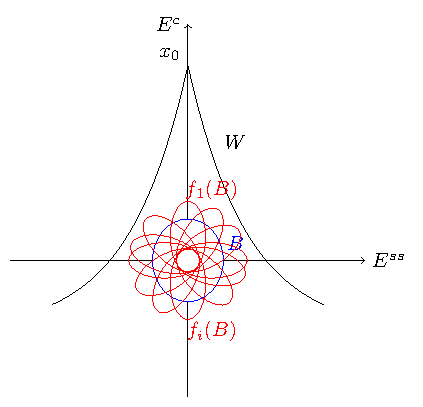
\includegraphics[scale=1.3]{new-fig.pdf}
\caption{\small{The covering property: The cusp-like region $W$ and the parabolic fixed point $x_0$ of $f$. The blending region $B$ and their images $f_i(B)$.}}\label{fig:2}
\vspace{-.5cm}
\end{center}
\end{figure}

Consider now the open ball $B=B(0,\delta)$, small $\delta >0$ with $B (0,5\delta)\subset \text{int}(W)$. Hence $x_0\not\in B$. See Figure \ref{fig:2}.
Consider now a contraction $g \in \mathrm{Inj}^2 (\mathbb{B}_n)$ whose restriction to the ball $B(0,4\,\delta)$ is given by
$$
g(x_1, \dots,x_n)= \frac{9}{10} (x_1,\dots, x_n) + (0,\dots,0, \delta/5).
$$
Then $p_\delta=(0, \dots, 0,2\,\delta)\not\in B$ is the fixed point of $g$,
the origin belongs to $g(B) \cap B$ (note that $g(0,\dots,0, -10\,\delta/45)=(0,\dots,0)$),
and a neighbourhood of the segment $\{0^{n-1}\} \times [0, \delta]$ is contained in $g(B) \cap B$. This implies that there is a family of linear isometries $A_2, \dots, A_k$ which fixes $0$ such that
\begin{equation}
\label{e.Biscontained}
B\subset \bigcup_{i=2}^k A_i(g(B)).
\end{equation}
By \cite{conradisometries}, if $A$ is an isometry of $\mathbb{R}^n$ that fixes 0 then there is an orthogonal decomposition $ \mathbb{R}^n = W_1 \bigoplus W_2 \bigoplus \dots \bigoplus W_m$ such that $dim(W_i) = 1$ or 2 for all $i$, and the restriction of $A$ to $W_i$ is a rotation unless $i = m$, $dim(W_m) = 1$, and $\text{det} A = -1$, in which case the restriction of $A$ to $W_m$ is a reflection.
For each $i$ let
$$
f_i = A_i \circ g \circ A_i^{-1}.
$$
The above fact implies that the map $f_i\in \mathrm{Inj}^2 (\mathbb{B}_n)$ is a contraction whose fixed point $A_i(p_\delta)$ has modulus $2\,\delta$ and hence does not belong to $B$.
In this way we obtain (H1)--(H3).

To complete (H4), note that $B=A_i (B)$, hence
$$
f_i(B) = A_i \circ g \circ A_i^{-1}(B) = A_i \circ g \circ A_i^{-1}(A_i(B)) = A_i (g (B)).
$$
Thus, by \eqref{e.Biscontained},
$$
B \subset \bigcup_{i=2}^k f_i(B).
$$
This implies that $B$ is a blending region disjoint from the fixed points of $f_1, \dots, f_k$, proving the theorem.
\end{proof}

According to the above arguments, we will have the following corollary.
\begin{corollary} \label{c.weakblending}
Consider a weakly attracting pair $(B,\mathcal{F})$, where $\mathcal{F}=\{f_1, \dots, f_k\}$.
Then there exist $C^2$ neighbourhoods $\mathcal{N}_i$ of $f_i$, $i=1, \dots, k$, such that for every family $\mathcal{G}=\{g_1, \dots, g_k\}$, with $g_i \in \mathcal{N}_i$, the pair $(B, \mathcal{G})$ satisfies conditions (H2)-(H4) in Definition~\ref{weakpair}.
Moreover, by Proposition \ref{open}, $g_1$ is either a weakly contractive map or a uniformly contracting map or it is normally contracting along some one dimensional submanifold of $\mathbb{B}_n$.
\end{corollary}



\section{Skew products and geometrical structures of their attracting invariant graphs}\label{sec3}

\subsection{Invariant graphs and maximal attractors}

As mentioned earlier, we now focus on skew products having non-uniform contraction rates along the fibers.
In what follows, we consider compact metric spaces $B$ and $Y$ and continuous maps $h \colon B \to B$.
Fixed $h$, as before, we denote by $\mathcal{C}_{h,\Lip}(B\times Y)$ the set of skew products
\begin{equation}
\label{e.asin}
F=F_{(h,f_b)} \colon B\times Y \to B \times Y, \qquad
F(b,y) =(h(b), f_b(y)),
\end{equation}
whose fiber maps $f_b$, $b \in B$, are Lipschitz and continuously depend on $b$.
In what follows, we let
$$
\Delta (Y) : = \{(y,y') \in Y \times Y \colon y\ne y' \}.
$$

\begin{definition}[Contracting on average, \cite{stark1999regularity}]\label{average}
Consider a skew product $F_{(h, f_b)}$ as above and a $h$-invariant measure $m$. We say that $F$ is \emph{$m$-contracting on average} if the limit
\begin{equation}\label{777}
\lambda(b) : = \lim_{n \to \infty}\frac{1}{n}\sup_{(y,y^{\prime})\in \Delta (Y)}\log \frac{d(f_b^n(y), f_b^n(y^{\prime}))}{d(y,y^{\prime})},
\end{equation}
exists for $m$-almost every $b$, the map $b \mapsto \lambda(b)$ is measurable, and there is $\lambda<0$ such that
\begin{equation}\label{landa}
 \lambda(b)\leq \lambda, \quad \text{for $m$-almost every $b$.}
\end{equation}
\end{definition}

In our context, the importance of the contracting on average property is illustrated by the following theorem.

\begin{theorem}{\em{(\cite[Theorem 1.4]{stark1999regularity})}}\label{thmg}
Consider compact metric spaces $B$ and $Y$, a homeomorphism $h\colon B \to B$, a $h$-invariant ergodic measure $m$, and an $m$-contracting on average skew product $F\in \mathcal{C}_{h, \Lip}(B\times Y)$.
Then there exist a $h$-invariant set $\Lambda \subset B$ with $m(\Lambda)= 1$ and a function $\gamma \colon \Lambda \to Y$ whose graph is invariant and attracting under $F$.
\end{theorem}

Denote by
\begin{equation}\label{ccc}
 \mathcal{C}^2_h(B \times Y)\subset \mathcal{C}_{h, \Lip} (B\times Y)
\end{equation}
the set of skew products whose fiber maps $f_b$, $b \in B$, are $C^2$ and continuously depend on $b$ with respect to $C^2$ topology.

\begin{lemma}\label{cor0}
Let $F=F_{(h,f_b)} \in \mathcal{C}^2_h(B \times Y)$ be a $m$-contracting on average skew product with respect to a $h$-invariant ergodic measure $m$.
Then there exists an open neighborhood $\mathcal{V}(F) \subset \mathcal{C}^2_h(B \times Y)$ of $F$ consisting of $m$-contracting on average skew products.
\end{lemma}

\begin{proof}
Since the map $(b,y)\mapsto f_b(y)$ is continuous and $C^2$ in $y$, there exists $\varsigma \in L^1(B,m)$ such that
\begin{equation*}
    d(f_b(y),f_b(y^{\prime}))<\varsigma(b)\,d(y,y^{\prime}),
\end{equation*}
for $m$-almost every $b$.
Then, by \cite[Lem.~5.1]{stark1999regularity}, for every $n\geq 0$ the number
\begin{equation}\label{n-lya}
\varsigma_{{F},n}(b)\eqdef \varsigma_n(b) \eqdef \sup_{(y,y^{\prime})\in \Delta (Y)}\frac{d(f_b^n(y) , f_b^n(y^{\prime}))}{d(y,y^{\prime})}
\end{equation}
exists for almost every $b$ and the map $\varsigma_n$ is measurable.
Also, by \cite[Lem.~5.3]{stark1999regularity}, the sequence $\varsigma_n$ is submultiplicative and hence $\log \varsigma_n$ is subadditive, that is,
$$
\log \varsigma_{n+m}(b)\leq \log \varsigma_n(b)+ \log \varsigma_m(h^n(b)).
$$
We can thus apply Kingman's subadditive ergodic theorem \cite[Thm.~5.4]{krengel2011ergodic} to $\log \varsigma_n$, obtaining that the map
\begin{equation}\label{lya}
\lambda(b)=\lim_{n \to +\infty}\frac{1}{n}\log \varsigma_n(b)
\end{equation}
exists for $m$-almost every $b$ and is $h$ invariant. Moreover, by subadditivity,
\begin{equation}\label{44}
\lim_{n \to \infty}\frac{1}{n}\log \varsigma_n(b)= \inf_{n}\frac{1}{n}\log \varsigma_n(b)
\end{equation}
and, by ergodicity of $m$, it is constant $m$-a.e., say equal to $\lambda_{F}$.
Since ${F}$ is contracting on average we have that $\lambda_{{F}} <0$.
Fix small $\delta>0$ and take any ${G}={G}_{(h,g_b)} \in \mathcal{C}^2_{h}(B\times Y)$ that is $\delta$-close to ${F}$ with respect to the metric in (\ref{e113}), that is, $\sup_{b} \text{dist}_{C^2}(f_b^{\pm}, g_b^{\pm})< \delta$.
We claim that, for small $\delta$, $G$ is contracting on average with respect to $m$. Indeed, as above, the sequence
\begin{equation}\label{per}
\varsigma_{{G},n} (b)\eqdef \sup_{(y,y^{\prime}\in \Delta (Y))}\frac{d(g_b^n(y) , g_b^n(y^{\prime}))}{d(y,y^{\prime})}.
\end{equation}
is subadditive and hence both statements (\ref{lya}) and (\ref{44}) hold for $\log \varsigma_{{G},n}$ (where in (\ref{lya}) we consider $\lambda_G(b)$).
In particular, by the ergodicity of $m$,
$$
\lim_{n \to +\infty}\frac{1}{n}\log \varsigma_{{G},n}(b)= \inf_{n}\frac{1}{n}\log \varsigma_{{G},n}(b)
$$
is constant $m$-a.e., say equal to $\lambda_{{G}}$. To prove the lemma, we need to see that $\lambda_{{G}}<0$.
Fix small $\varepsilon>0$ with $\lambda_{{F}}+2\varepsilon <0$.
By \eqref{44}, $\lambda_{{F}}=\inf_{n}\frac{1}{n}\log \varsigma_n(b)$, for $m$-a.e. $b$. Thus, for a typical point $b$ for $\lambda_{{F}}$ and $\lambda_{{G}}$, there exists $n_0=n_0(b) \in \mathbb{N}$ such that
$$
\frac{1}{n_0}\log \varsigma_{{F}, n_0}(b)< \lambda_{{F}}+\varepsilon.
$$
Taking $\delta$ small enough, we get
$$
\frac{1}{n_0}\log \varsigma_{{G},n_0}(b)< \lambda_{{F}}+2 \varepsilon <0.
$$
Consequently,
$$
\lambda_{{G}}=\inf_{n}\frac{1}{n}\log \varsigma_{G,n}< \frac{1}{n_0}\log \varsigma_{G,n_0}(b)< \lambda_{{F}} + 2\varepsilon <0,
$$
proving that ${G}$ is contracting on average with respect to $m$.
\end{proof}

In this section, we introduce a class of skew products driven by an expanding circle map and their solenoidal extensions. We show that maximal attractors of the extension skew products are either an attracting continuous invariant graph or a thick $n$-porcupine graph.

\subsection{Skew products driven by expanding circle maps and their extensions}\label{section}

Given $\ell\in \mathbb{N}$, $\ell\ge 2$, we consider the expanding map of the circle
$$
\varphi_\ell \colon \mathbb{T}^1 \to \mathbb{T}^1,\quad \varphi_\ell (t) = \ell t \ (\mathrm{mod\, 1}).
$$
Take skew product maps defined on $\mathbb{T}^1\times \mathbb{B}_n$ driven by $\varphi_\ell$ of the form
\begin{equation}\label{skewT1}
 F_{(\ell, f_t)} \colon \mathbb{T}^1\times \mathbb{B}_n \to \mathbb{T}^1\times \mathbb{B}_n, \quad F (t,x)=(\varphi_\ell(t), f_t(x)),
\end{equation}
where the fiber maps $f_t \colon \mathbb{B}_n \to \mathbb{B}_n$, $t \in \mathbb{T}^1$, are $C^2$ diffeomorphisms from the compact ball $\mathbb{B}_n$ onto their images such that $f_t(\mathbb{B}_n)\subset \text{int}(\mathbb{B}_n)$.
Since the maps $\varphi_\ell$ are not invertible, we consider their extensions given by the inverse limit construction in \cite{williams1974expanding}.
For that consider the set
$$
\mathcal{S}_\ell :=\{(\ldots,t_{-1},t_{0})\in (\mathbb{T}^1)^{\mathbb{Z}^-}: t_{-j}=\varphi_\ell (t_{-j-1})\}
$$
endowed with the product topology. The extension $\xi_\ell$ of $\varphi_\ell$ is defined by
\begin{equation*}\label{3.9}
\xi_\ell \colon \mathcal{S}_\ell \to \mathcal{S}_\ell, \quad \xi(\textbf{t})=(\ldots,t_{-1},t_{0},\varphi_\ell(t_0)), \ \textnormal{for} \ \textbf{t}=(\ldots,t_{-1},t_{0}).
\end{equation*}
The extension map $\xi_\ell$ is invertible and its inverse is given by
\begin{equation*}
\xi_\ell^{-1}(\textbf{t})=(\ldots,t_{-2},t_{-1}).
\end{equation*}
Finally, consider the projection
\begin{equation}\label{e99}
\pi_\ell \colon \mathcal{S}_\ell \rightarrow \mathbb{T}^1, \quad \pi(\textbf{t})=t_0.
\end{equation}
Note that $\pi_\ell \circ \xi_\ell=\varphi_\ell \circ \pi_\ell$, which means that $\pi_\ell$ is a semiconjugacy between $\varphi_\ell$ and $\xi_\ell$.
The skew product map $F_{(\ell, f_t)}$ in \eqref{skewT1} induces the skew product map $\mathbb{F}_{F}=\mathbb{F}_{(\xi_\ell, f_{\textbf{t}})}$ on $\mathcal{S}_\ell \times \mathbb{B}_n$, called the \emph{extension of $F$}, defined by
\begin{equation}\label{skew4}
\mathbb{F}_{F}(\textbf{t},x)=(\xi_\ell(\textbf{t}),f(\textbf{t},x))=(\xi_\ell(\textbf{t}),f_{\textbf{t}}(x)),
\end{equation}
where $f_{\textbf{t}}(x):=f_{t_0}(x)$.

\begin{remark}\label{rem90}
The fiber maps of the skew product maps $F_{(\ell, f_t)}$ and $\mathbb{F}_{F}$ are the same.
\end{remark}

\begin{remark}\label{circ-measure}
On the circle $\mathbb{T}^1$ and the inverse limit spaces $\mathcal{S}_\ell$, we use Borel $\sigma$-algebras.
Note that the expanding map $\varphi_\ell$ possesses an absolutely continuous invariant ergodic measure $\nu_\ell^+$ whose density is bounded away from zero and is equivalent to Lebesgue \cite{krzyzewski2004invariant, mane2012ergodic}.
The extension map $\xi_\ell$ has the invariant measure $\nu_\ell$ defined on $\mathcal{S}_\ell$ inherited from $\nu_\ell^+$ defined by
\begin{equation*}
  \nu_\ell (\{t_{-n}\in I_n, \cdots, t_0 \in I_0\}) : =\nu_\ell^+(\varphi_\ell^{-n}(I_0) \cap \varphi_\ell^{-n+1}(I_1)\cap \cdots \cap I_n),
\end{equation*}
where $I_i$, $i=0, \cdots, n,$ are intervals of $\mathbb{T}^1$.
\end{remark}

\begin{notations}\label{n.espacesofmaps}
The following notations are introduced:
\begin{enumerate}
  \item The space of all skew products $F_{(\ell, f_t)}$ as in \eqref{skewT1} is denoted by $\mathcal{C}_\ell(\mathbb{T}^1\times \mathbb{B}_n)$.
  We denote by $\mathcal{C} (\mathcal{S}_\ell \times \mathbb{B}_n)$ the space of skew product maps $\mathbb{F}= \mathbb{F}_{F}$ which are an extension of some $F\in \mathcal{C}_\ell(\mathbb{T}^1\times \mathbb{B}_n)$.
  We equip these spaces with the metric given by \eqref{e113}
  \item Given $F_{(\ell, f_t)}$, the set of all $F$-invariant probability measures on $\mathbb{T}^1\times \mathbb{B}_n$ with marginal $\nu_\ell^+$ is denoted by $\mathcal{M}_{\nu_\ell^+}(F)$.
  \item Similarly, for $\mathbb{F}= \mathbb{F}_{F}$, we denote by $\mathcal{M}_{\nu_\ell}(\mathbb{F})$ the set of all $\mathbb{F}$-invariant probability measures on $\mathcal{S}_\ell\times \mathbb{B}_n$ with marginal $\nu_\ell$.
\end{enumerate}
\end{notations}

We equip the space $\mathcal{C}_\ell(\mathbb{T}^1\times \mathbb{B}_n)$ with the following metric:
\begin{equation}\label{e113}
  \textnormal{dist}_{ \mathcal{C}_{\ell}}(F,G):=\sup_{t \in \mathbb{T}^1}(\textnormal{dist}_{C^2}(f_t^{\pm 1} , g_t^{\pm 1})), \ \textnormal{for each } F,G \in \mathcal{C}_\ell(\mathbb{T}^1\times \mathbb{B}_n).
\end{equation}
The following lemma \cite{crauel1990extremal} relates invariant measures for a skew product and its extension.

\begin{lemma}[\cite{crauel1990extremal} and Lemma 2.1 in \cite{homburg2012circle}] \label{L1.1}
Let $F_{(\ell, f_t)}$ and consider any invariant measure $\mu^+ \in \mathcal{M}_{\nu_\ell^+}(F)$ with disintegration $(\mu^+_{{t}})_{t\in \mathbb{T}^1}$.
Then there is an invariant measure $\mu \in \mathcal{M}_{\nu_\ell}(\mathbb{F}_{F})$ whose disintegration $(\mu_{\textbf{t}})_{\textbf{t} \in \mathcal{S}_\ell}$ is given by
\begin{equation*}
  \mu_\textbf{t}=\lim_{n \to \infty}f^n_{t_{-n}}\mu^+_{t_{-n}}
\end{equation*}
for $\nu_\ell$-almost every $(\ldots,t_{-1},t_{0})\in \mathcal{S}_\ell$.
\end{lemma}

\subsection{The subset $\mathcal{A}_{\ell,\mathbb{T}^1} = \mathcal{A}_\ell (\mathbb{T}^1 \times \mathbb{B}_n)$ of $\mathcal{C}_\ell(\mathbb{T}^1 \times \mathbb{B}_n)$}

In what follows, we define the subset $\mathcal{A}_{\ell, \mathbb{T}^1} $.

\begin{definition}[The sets $\mathcal{A}_{\ell, \mathbb{T}^1}$ and $\mathcal{A}_{\mathcal{S}_\ell}$]\label{ourconditions}
Given $\ell \ge 2$, denote by $\mathcal{A}_{\ell, \mathbb{T}^1} =\mathcal{A}_\ell (\mathbb{T}^1 \times \mathbb{B}_n)$ the subset of $\mathcal{C}_\ell(\mathbb{T}^1 \times \mathbb{B}_n)$ consisting of all skew product maps $F_{(\varphi_\ell, f_t)}$ which are contracting on average with respect to the measure $\nu^+_\ell$ and such that there are an open ball $B \subset \mathrm{int}(\mathbb{B}_n)$, disjoint closed intervals $\{L_{1}, \dots, L_{k}\}$ of $\mathbb{T}^1$, with $\ell/2 \ge k \ge 3$, and a family $\mathcal{F}=\{f_{t_1}, \dots, f_{t_k}\}$ of fiber maps of $F$ with $t_i\in L_i$ for every $i=1,\dots, k$ such that:
\begin{enumerate}
  \item [(A1)] $(B,\mathcal{F})$ is a weak attracting pair.
   \item [(A2)]
   \begin{enumerate}
    \item [(i)] $f_1\in\mathbb{WC}^2 ( \mathbb{B}_n)$ and there is a normally hyperbolic adapted $C^2$ neighborhood $\mathcal{N}_{f_1}$ of $f_1$ (see Definition \ref{nhyper}) such that $f_t \in \mathcal{N}_{f_1}$ for every $t \in L_1$,
      \item [(ii)] for every $s_i \in L_i$, $i=2, \ldots, k$, the fiber maps $\{f_{s_2}, \ldots, f_{s_k}\}$ satisfy the covering property
    $$
\mathrm{clos}(B)\subset f_{s_2}(B)\cup \cdots \cup f_{s_k}(B);
$$
\item[(iii)] for every $t\not\in L_1$ the fiber map $f_t$ of $F$ is uniformly contracting.
  \end{enumerate}
  \item [(A3)] $\varphi_\ell (L_i)=\mathbb{T}^1$ for every $i=1, \dots, k$.
     \end{enumerate}
We define the subset $\mathcal{A}_{\mathcal{S}_\ell} =\mathcal{A} (\mathcal{S}_\ell \times \mathbb{B}_n)$ of $\mathcal{C}(\mathcal{S}_\ell \times \mathbb{B}_n)$ as follows:
 $$
 \mathcal{A}_{\mathcal{S}_\ell} \eqdef \big\{\mathbb{F}=\mathbb{F}_{F} \in \mathcal{C}(\mathcal{S}_\ell \times \mathbb{B}_n) \,\ , \text{such \ that } F \in \mathcal{A}_{\ell ,\mathbb{T}^1}\big\}.
$$
\end{definition}

In Section \ref{assp}, we will show that the sets $\mathcal{A}_{\ell, \mathbb{T}^1}$ (and hence the sets $\mathcal{A}_{\mathcal{S}_\ell}$) are not empty for every $\ell$ large enough.

\begin{theorem}\label{thm1}
For every $\ell$ sufficiently large, there is an open neighbourhood $ \mathcal{V}_{\mathcal{S}_\ell}$ of $ \mathcal{A}_{\mathcal{S}_\ell}$ in $\mathcal{C}(\mathcal{S}_\ell \times \mathbb{B}_n)$ such that every $\mathbb{F}\in \mathcal{V}_{\mathcal{S}_\ell}$ has a maximal attractor $A_{max}(\mathbb{F})$ that is topologically transitive and satisfies the following dichotomy:
 \begin{enumerate}
   \item [$-$] either $A_{max}(\mathbb{F})$ is an attracting continuous invariant graph;
   \item [$-$] or $A_{max}(\mathbb{F})$ is a solenoidal $n$-porcupine-like graph.
      \end{enumerate}
 \end{theorem}

The proof of this theorem is given in Subsection~\ref{complete}.
By Lemma \ref{cor0}, to be contracting on average is an open condition. So, fixed $\ell$, we can take an open set $\mathcal{W}_{\ell, \mathbb{T}^1} \supset \mathcal{A}_{\ell, \mathbb{T}^1}$ consisting of skew product maps $F_{(\varphi_\ell, f_t)}$ which are contracting on average with respect to $\nu^+_\ell$.
We let
\begin{equation}\label{vopen}
 \mathcal{W}_{\mathcal{S}_\ell} \eqdef \big\{\mathbb{F}=\mathbb{F}_{F} \in \mathcal{C}(\mathcal{S}_\ell \times \mathbb{B}_n) \,\ , \text{such \ that } F \in \mathcal{W}_{\ell, \mathbb{T}^1}\big\}.
\end{equation}

\begin{remark}\label{remopen}
Since $\pi_\ell$, given by \eqref{e99}, is a semiconjugacy between $\varphi_\ell$ and $\xi_\ell$, and by Remark \ref{rem90}, the fiber maps of $F$ and $\mathbb{F}=\mathbb{F}_{F}$ are the same, thus, $\mathcal{W}_{\mathcal{S}_\ell}$ is open in $\mathcal{C}(\mathcal{S}_\ell \times \mathbb{B}_n)$.
\end{remark}

Consider $\mathbb{F} = \mathbb{F}_{(\xi_\ell, \textbf{f}_{\textbf{t}})} \in \mathcal{W}_{\mathcal{S}_\ell}$.
By definition, $\mathbb{F}$ is contracting on average with respect to $\nu_\ell$.
Since $\mathcal{S}_\ell$ and $\mathbb{B}_n$ are compact metric spaces, $\xi_\ell$ is a homeomorphism, $\nu_\ell$ is an invariant ergodic measure, and the fiber maps $f_{\textbf{t}}$ are $C^2$ diffeomorphisms onto their images, we can apply Theorem \ref{thmg} to $\mathbb{F}$, getting the next result.

\begin{proposition}\label{p.thm000}
Let $\mathbb{F}\in \mathcal{W}_{\mathcal{S}_\ell}$.
Then there exist a $\xi_\ell$-invariant set $\widetilde{\mathcal{S}}_\ell\subseteq \mathcal{S}_\ell$ with $\nu_\ell(\widetilde{\mathcal{S}}_\ell )=1$ and a measurable function $\gamma_{\mathbb{F}} \colon \widetilde{\mathcal{S }}_\ell\to \mathbb{B}_n$ whose graph is invariant and attracting under $\mathbb{F}$.
\end{proposition}

\subsection{Skew products with high dimensional porcupine graph}\label{complete}

By shrinking the set $\mathcal{W}_{\ell, \mathbb{T}^1}$, we may assume that every fiber map $f_t$ of any $F \in \mathcal{W}_{\ell, \mathbb{T}^1}$ belongs to $\text{Inj}^2(\mathbb{B}_n)$.
By Remark \ref{rem90}, the same holds for any $\mathbb{F}=\mathbb{F}_{F} \in \mathcal{W}_{\mathcal{S}_\ell}$.
This implies that $\mathcal{S}_\ell \times \mathbb{B}_n$ is a trapping region of $\mathbb{F}$, hence its maximal attractor
\begin{equation}\label{e67}
  A_{max}(\mathbb{F})\eqdef \bigcap_{n\geq 0}\mathbb{F}^n(\mathcal{S_\ell} \times \mathbb{B}_n)
\end{equation}
is well defined.
In what follows, the integer $\ell$ remains fixed and hence the subscript $\ell$ will be omitted.

\begin{proof}[Proof of Theorem \ref{thm1}]
Take $\mathbb{F}=\mathbb{F}_{F} \in \mathcal{W}_{\mathcal{S}_\ell}$.
By Proposition~\ref{p.thm000}, there are a $\xi$-invariant set $\widetilde{\mathcal{S}}\subset \mathcal{S}$ with $\nu(\widetilde{\mathcal{S}}) = 1$ and a measurable function $\gamma_{\mathbb{F}} : \widetilde{\mathcal{S}}\to \mathbb{B}_n$ whose graph $\gamma_{\mathbb{F}}$, denoted by $\Gamma_{\mathbb{F}}$, is $\mathbb{F}$-invariant.

\begin{lemma}\label{inclusion}
Let $\mathbb{F}=\mathbb{F}_{F} \in \mathcal{W}_{\mathcal{S}_\ell}$.
Then $\Gamma_{\mathbb{F}} \subset A_{max}(\mathbb{F})$. Moreover, if $\widetilde{\mathcal{S}}=\mathcal{S}$ then $\Gamma_{\mathbb{F}}= A_{max}(\mathbb{F})$.
\end{lemma}

\begin{proof}
For each $\textbf{t}=(\ldots, t_{-n}\ldots, t_{-1}, t_0)\in \mathcal{S}$ define
\begin{equation}\label{nested}
 \mathbb{B}^k(\textbf{t},\mathbb{F})\eqdef f_{\xi_\ell^{-1}(\textbf{t})}\circ \dots \circ f_{\xi_\ell^{-k}(\textbf{t})}(\mathbb{B}_n)=f_{t_{-1}}\circ \dots \circ f_{t_{-k}}(\mathbb{B}_n).
\end{equation}
As the fiber maps $f_{t_{-j}}$ belong to $\text{Inj}^2(\mathbb{B}_n)$ the sets $\mathbb{B}^k(\textbf{t},\mathbb{F})$ are well defined and form a nested sequence of compact sets. Thus,
  \begin{equation}\label{nonempty}
  \mathbb{B}^{\infty}(\textbf{t},\mathbb{F})\eqdef \bigcap_{k=0}^\infty \mathbb{B}^k(\textbf{t},\mathbb{F})\neq \emptyset.
  \end{equation}
Note that
\begin{equation}\label{aa}
A_{max}(\mathbb{F}) \bigcap (\{\textbf{t}\} \times \mathbb{B}_{n}) = \mathbb{B}^{\infty}(\textbf{t},\mathbb{F}).
\end{equation}
Note that, $\Gamma_{\mathbb{F}}$ is attracting, so, for each $\textbf{t} \in \widetilde{\mathcal{S}}$,
$$
\lim f_{\xi_\ell^{-1}(\textbf{t})}\circ \dots \circ f_{\xi_\ell^{-n}(\textbf{t})}(\mathbb{B}_n)=\lim f_{\xi_\ell^{-1}(\textbf{t})}\circ \dots \circ f_{\xi_\ell^{-n}(\textbf{t})}( \gamma_\mathbb{F}(\textbf{t}))= B^\infty(\textbf{t} , \mathbb{F}).
$$
Since the graph $\gamma_{\mathbb{F}}$ is invariant, we get
$$
\Gamma_\mathbb{F} = \bigcup_{\textbf{t} \in \widetilde{\mathcal{S}}} B^\infty(\textbf{t} , \mathbb{F}) \subset A_{max}(\mathbb{F}),
$$
proving the first part of the lemma.
For the second part, assuming that $\widetilde{\mathcal{S}}= \mathcal{S}$, note that by \eqref{aa} it holds
$$
A_{max}(\mathbb{F}) = \bigcup_{\textbf{t} \in {\mathcal{S}}} \Big( A_{max}(\mathbb{F}) \cap \big( \{\textbf{t}\} \times \mathbb{B}_n \big) \Big) = \bigcup_{\textbf{t} \in {\mathcal{S}}} \{\textbf{t}\} \times \mathbb{B}^\infty (\textbf{t},\mathbb{F})= \Gamma_\mathbb{F},
$$
which ends the proof of the lemma.
\end{proof}

By Lemma~\ref{inclusion}, if $\widetilde{\mathcal{S}}=\mathcal{S}$ then $A_{max}(\mathbb{F})$ is an invariant graph and the graph function $\gamma_{\mathbb{F}}$ is defined on the whole space $\mathcal{S}$.
In this case, we have $\Gamma_{\mathbb{F}} = A_{max}(\mathbb{F})$.
For the case that $\widetilde{\mathcal{S}}\neq\mathcal{S}$, the lemma below states the structure of non-trivial spines.

\begin{lemma}\label{tangent}
Let $\mathbb{F} \in \mathcal{W}_{\mathcal{S}_\ell}$ and there exist $\textbf{t} \in \mathcal{S} \setminus \widetilde{\mathcal{S}}$ for that $ \mathbb{B}^{\infty}(\textbf{t},\mathbb{F})$ is nontrivial.
Then the set $ \mathbb{B}^{\infty}(\textbf{t},\mathbb{F})$ is a one dimensional submanifold tangent to the central bundle.
\end{lemma}

\begin{proof}
Let $\mathbb{F}=\mathbb{F}_{F} \in \mathcal{W}_{\mathcal{S}_\ell} $ with nontrivial spine $ \mathbb{B}^{\infty}(\textbf{t},\mathbb{F})$, for $\textbf{t} \in \mathcal{S} \setminus \widetilde{\mathcal{S}}$. Then $F \in \mathcal{W}_{\ell, \mathbb{T}^1} $.
By item $(iii)$ of Condition ($A2$) of Definition \ref{ourconditions} and shrinking $\mathcal{W}_{\ell, \mathbb{T}^1} $, for each $t \in \mathbb{T}^1 \setminus L_1$, the fiber maps $f_t$ of $F$ are uniformly contracting.
By Remark \ref{rem90}, the fiber maps of $\mathbb{F}_{F}$ and $F$ are the same.
So, this fact holds for every $\mathbb{F} \in \mathcal{W}_{\mathcal{S}_\ell} $ and every $\textbf{t}=(\dots, t_{-1}, t_0) \in \mathcal{S} $ with $t_0 \in \mathbb{T}^1 \setminus L_1 $.
Given $\textbf{t}=(\dots, t_{-1}, t_0) \in \mathcal{S} $, define
 \begin{equation*}
    n(\textbf{t})\eqdef \sup \{j: t_{-j} \in \mathbb{T}^1 \setminus L_1\}.
   \end{equation*}
If $n(\textbf{t})$ is finite, then for each $j > n(\textbf{t})$, $t_{-j}\in L_1$.
Therefore, By item $(i)$ of Condition ($A2$) of Definition \ref{ourconditions} and Proposition \ref{open}, the intersection $\bigcap_{m\geq 0} \mathbb{B}^m(\textbf{t},\mathbb{F})=\lim_{n \to \infty}f_{t_{-1}}\circ \dots \circ f_{t_{-m}}(\mathbb{B}_n)$ is either a single point or a one dimensional $C^1$ submanifold.
 The hypothesis that $ \mathbb{B}^{\infty}(\textbf{t},\mathbb{F})$ is nontrivial, prevents the first case.
So, $ \mathbb{B}^{\infty}(\textbf{t},\mathbb{F})$ is a one dimensional $C^1$ submanifold.
Now, assume that $n(\textbf{t})$ is infinite. If the set $\{j: t_{-j} \in L_1\}$ is finite, a straightforward argument shows that $ \mathbb{B}^{\infty}(\textbf{t},\mathbb{F})$ is a single point that contradicts the hypothesis. So, the set $\{j: t_{-j} \in L_1\}$ is infinite. This means that there are infinitely many $t_{-j} \in L_1$ and also infinitely many $t_{-j} \in \mathbb{T}^1 \setminus L_1$. In this case, the proof follows from Theorem \ref{open2} and the hypothesis that $ \mathbb{B}^{\infty}(\textbf{t},\mathbb{F})$ is nontrivial.
 \end{proof}

 Note that
$$
A_{max}(\mathbb{F})=\bigcup_{\textbf{t} \in \mathcal{S}}\mathbb{B}^{\infty}(\textbf{t},\mathbb{F}).
$$

\begin{lemma}\label{corspine}
Let $\mathbb{F} \in \mathcal{W}_{\mathcal{S}_\ell}$ and suppose that there exists a nontrivial spine $ \mathbb{B}^{\infty}(\textbf{t},\mathbb{F})$, for some $\textbf{t} \in \mathcal{S}$. Then the set of nontrivial spines has the cardinality of the continuum and it is dense in $\mathcal{S}$. Furthermore, the same holds for the set $\widetilde{\mathcal{S}}$.
\end{lemma}

\begin{proof}
For $t_j \in \mathbb{T}^1$, $j=1, \dots, m$, we denote by $\bar t(m)=(t_1, \dots, t_m)$.
Define
$$\mathrm{dist} (\bar t(m) , \bar t'(m))\eqdef \max \{d_{\mathbb{T}^1}(t_1,t^{\prime}_1), \dots, d_{\mathbb{T}^1}(t_m,t^{\prime}_m) \},$$
where $\bar t(m)=(t_1, \dots, t_m)$ and $\bar t^{\prime}(m)=(t^{\prime}_1, \dots, t^{\prime}_m)$. Also, given $t_j \in \mathbb{T}^1$, $j=1, \dots, m$, denote by $f_{[\bar t(m)]}\eqdef f_{[t_1, \dots, t_m]}\eqdef f_{t_1} \circ \dots \circ f_{t_m}$.

\begin{claim}\label{c2121}
For every $m \geq 1$ and $\varepsilon > 0$ there exists $\delta =\delta(m, \varepsilon)> 0$ such that for every $t_j, t^{\prime}_j \in \mathbb{T}^1$, $j=1, \dots, m$, with
\begin{equation*}
  \mathrm{dist} (\bar t(m) , \bar t'(m)) < \delta
\end{equation*}
then
\begin{equation*}
  |\text{diam}(f_{[\bar t(m)]}(\mathbb{B}_n)) - \text{diam}(f_{[\bar t^{\prime}(m)]}(\mathbb{B}_n))|< \varepsilon.
\end{equation*}
\end{claim}

\begin{proof}
Fix any $m \in \mathbb{N}$ and $\varepsilon>0$. Since the map $(\bar t(m),y)\mapsto f_{[\bar t(m)]}(y)$ is uniformly continuous, thus, there exists $\delta > 0$ such that for each $t_j, t^{\prime}_j \in \mathbb{T}^1$, $j=1, \dots, m$,
$$ \max \{\mathrm{dist} (\bar t(m) , \bar t'(m)),d_{\mathbb{B}_n}(x,y) \} < \delta, \quad \text{implies \ that } \quad d_{\mathbb{B}_n}(f_{[\bar t(m)]}(x) , f_{[\bar t^{\prime}(m)]}(y))<\varepsilon/2.$$
Take $\bar t(m)= (t_1, \dots, t_m)$ and $\bar t'(m)=(t^{\prime}_1, \dots, t^{\prime}_m)$ in $\mathbb{T}^m$ such that $ \mathrm{dist} (\bar t(m) , \bar t'(m)) < \delta$. For $A \subseteq \mathbb{B}_n$, let $U_{\varepsilon /2}(A) \eqdef \{y \in \mathbb{B}_n : d_{\mathbb{B}_n}(y,A)\leq \varepsilon /2\}$.
We need to show that
\begin{equation}\label{inc}
f_{[\bar t(m)]}(\mathbb{B}_n)\subset U_{\varepsilon/2}(f_{[\bar t^{\prime}(m)]}(\mathbb{B}_n)) \quad \text{and} \quad f_{[\bar t^{\prime}(m)]}(\mathbb{B}_n)\subset U_{\varepsilon/2}(f_{[\bar t(m)]}(\mathbb{B}_n)).
\end{equation}
This implies that
$$\text{diam}(f_{[\bar t(m)]}(\mathbb{B}_n))\leq \text{diam}(f_{[\bar t^{\prime}(m)]}(\mathbb{B}_n)) + \varepsilon \quad \text{and} \quad \text{diam}(f_{[\bar t^{\prime}(m)]}(\mathbb{B}_n))\leq \text{diam}(f_{[\bar t(m)]}(\mathbb{B}_n)) + \varepsilon,$$ proving the claim.
We now prove \eqref{inc}. Given $y \in f_{[\bar t(m)]}(\mathbb{B}_n)$ we can write $y=f_{[\bar t(m)]}(x)$ for some $x \in \mathbb{B}_n$. Hence, taking $y^{\prime}=f_{[\bar t^{\prime}(m)]}(x)$, we have
\begin{equation*}
  d_{\mathbb{B}_n}(y,y^{\prime})=d_{\mathbb{B}_n}(f_{[\bar t(m)]}(x),f_{[\bar t^{\prime}(m)]}(x))<\varepsilon/2,
\end{equation*}
proving that $y \in U_{\varepsilon/2}(f_{[\bar t^{\prime}(m)]}(\mathbb{B}_n))$. The proof of the other inclusion of (\ref{inc}) is similar.
\end{proof}

In what follows, for each $\textbf{t} = (\ldots , t_{-m},\ldots , t_{-1}, t_{0}) \in \mathcal{S} $ the finite word $\tilde{t}(m) = (t_{-1},\ldots , t_{-m})$ is called the corresponding $m$-word of $\textbf{t}$.
Let us take the disjoint closed intervals $I_i \subset \mathbb{T}^1$, $i=1, \dots, \ell$, with length $1/ \ell$, such that $\mathbb{T}^1=\bigcup_{i=1}^\ell I_i$ and there exist indices $i_j$, $j=1, \dots, k$, so that $I_{i_j}=L_j$, where $L_j$ are disjoint closed intervals of $\mathbb{T}^1$ given by Definition \ref{ourconditions}.
Then by the choice of $I_{i}$ , $\varphi_\ell (I_i)=\mathbb{T}^1$.
Fix any $\textbf{t}=(\dots, t_{-1}, t_0) \in \mathcal{S}$ for that $\mathbb{B}^{\infty}(\textbf{t},\mathbb{F})$ is a non-trivial spine.
Take $\varepsilon > 0$ with
\begin{equation}\label{m2}
\varepsilon <\frac{1}{8} \text{diam}(\mathbb{B}^{\infty}(\textbf{t},\mathbb{F})),
\end{equation}
and $m$ sufficiently large such that
\begin{equation}\label{m3}
U_{\varepsilon/2}( f_{[\bar t(m)]}(\mathbb{B}_n))\subset U_{\varepsilon}(\mathbb{B}^{\infty}(\textbf{t},\mathbb{F})).
\end{equation}
where $\tilde{t}(m) = (t_{-1}, \ldots , t_{-m})$ is the corresponding $m$-word of $\textbf{t}$.
By Claim \ref{c2121} and inclusions (\ref{inc}), for $\varepsilon$ given by (\ref{m2}) , there exists $\delta > 0$ such that for each $\textbf{t}^{\prime}=(\ldots, t^{\prime}_{-m}, \ldots, t^{\prime}_{-1}, t^{\prime}_0) \in \mathcal{S}$ and the corresponding $m$-word $\bar t^{\prime}(m)=(t^{\prime}_{-1}, \dots, t^{\prime}_{-m})$ of $\textbf{t}^{\prime}$ , if $ \max\{d_{\mathbb{T}^1}(t_0, t^{\prime}_0), {dist} (\bar t(m) , \bar t'(m))\} < \delta$ then
\begin{equation}\label{m1}
 f_{[\bar t(m)]}(\mathbb{B}_n)\subset U_{\varepsilon/2}(f_{[\bar t^{\prime}(m)]}(\mathbb{B}_n)), \quad f_{[\bar t^{\prime}(m)]}(\mathbb{B}_n)\subset U_{\varepsilon/2}(f_{[\bar t(m)]}).
\end{equation}
Now, we choose a sequence $\textbf{t}^{\prime}=(\ldots, t^{\prime}_{-n}\ldots, t^{\prime}_{-1}, t^{\prime}_0)\in \mathcal{S}$ with $d_{\mathbb{T}^1}(t_{0} , t^{\prime}_{0})<\delta$, so that for each $j$, $t_{-j}$ and $t^{\prime}_{-j}$ belong to the same closed interval $I_{i_j}$.
Since $\varphi_\ell(t_{-j-1})=t_{-j}$ and $\varphi_\ell(t^{\prime}_{-j-1})=t^{\prime}_{-j}$, hence $t_{-j-1}, t^{\prime}_{-j-1} \in \varphi^{-1}_\ell(I_j)$.
Note that the inverse branch $\varphi^{-1}_\ell|_{I_j}$ is a contraction with a uniform contracting rate $1/\ell$.
Thus, for each $j$, $d_{\mathbb{T}^1}(t_{-j-1} , t^{\prime}_{-j-1})< 1/\ell d_{\mathbb{T}^1}(t_{-j} , t^{\prime}_{-j})$.
Thus, for each $j$
\begin{equation}\label{dd1}
 d_{\mathbb{T}^1}(t_{-j} , t^{\prime}_{-j})<\delta,
\end{equation}
which implies that $\max\{d_{\mathbb{T}^1}(t_0, t^{\prime}_0), {dist} (\bar t(m) , \bar t'(m))\} < \delta.$
Then, by (\ref{m3}) , (\ref{m1}) and (\ref{dd1})
\begin{equation}\label{m30}
U_{\varepsilon/2}( f_{[\bar t^\prime(m)]}(\mathbb{B}_n))\subset U_{\varepsilon}(\mathbb{B}^{\infty}(\textbf{t}^\prime,\mathbb{F})).
\end{equation}
Therefore, by (\ref{m1}) and (\ref{m30})
\begin{equation}\label{m5}
\mathbb{B}^{\infty}(\textbf{t},\mathbb{F}) \subset f_{[\bar t(m)]}(\mathbb{B}_n)\subset U_{\varepsilon/2}(f_{[\bar t^{\prime}(m)]}(\mathbb{B}_n)) \subset U_{\varepsilon}(\mathbb{B}^{\infty}(\textbf{t}^{\prime},\mathbb{F})).
\end{equation}
Consequently, by \eqref{m5} and \eqref{m2}, we get
\begin{equation}\label{prime}
  \text{diam}(\mathbb{B}^{\infty}(\textbf{t},\mathbb{F}))\leq \text{diam}(\mathbb{B}^{\infty}(\textbf{t}^{\prime},\mathbb{F}))+2\varepsilon \leq \text{diam}(\mathbb{B}^{\infty}(\textbf{t}^{\prime},\mathbb{F})) + \frac{1}{4}\text{diam}(\mathbb{B}^{\infty}(\textbf{t},\mathbb{F})).
\end{equation}
By (\ref{prime}), since $\mathbb{B}^{\infty}(\textbf{t},\mathbb{F})$ is a non-trivial spine, $\mathbb{B}^{\infty}(\textbf{t}^{\prime},\mathbb{F})$ is also a nontrivial spine.
 As a result, the set of nontrivial spines has the cardinality of the continuum but it is not an open subset of $\mathcal{S}$.
Because, for each $t_0^{\prime}\in \mathbb{T}^1$ with $d_{\mathbb{T}^1}(t_{0} , t^{\prime}_{0})<\delta$ , there exists only one inverse limit branch $\textbf{t}^{\prime}=(\ldots, t^{\prime}_{-m}\ldots, t^{\prime}_{-1}, t^{\prime}_0)$ that fulfills the construction described above, namely, for each $j$, $t_{-j}$ and $t^{\prime}_{-j}$ belong to the same closed interval $I_{i_{j}}$.
To prove the next statement, take any $\textbf{t}^{\prime}$ with a nontrivial spine as above such that $t^{\prime}_{0}$ is irrational and let $\textbf{s}_k=\xi_\ell^k(\textbf{t}^{\prime})=(\dots, t^{\prime}_{-j}, \ldots, t^{\prime}_0, \varphi_\ell(t^{\prime}_0), \dots, \varphi_\ell^k(t^{\prime}_0))$, for each positive integer $k$.
Then, by continuity, for each $k\geq 1$, we have
$$\lim_{m \to \infty}f_{[\bar s_k(k+m)]}(\mathbb{B}_n)=\lim_{m \to \infty} f_{\varphi_\ell^k(t^{\prime}_0)}\circ \dots \circ f_{t^{\prime}_0}\circ \dots \circ f_{t^{\prime}_{-m}}(\mathbb{B}_n)= f_{\varphi_\ell^k(t^{\prime}_0)}\circ \dots \circ f_{\varphi_\ell(t^{\prime}_0)} (\lim_{m \to \infty} f_{[\bar t^{\prime}(m)]}(\mathbb{B}_n)).$$
Consequently, $\mathbb{B}^{\infty}(\textbf{s}_k,\mathbb{F})$ is a non-trivial spine.
Since $t_0^{\prime}$ is irrational, the $\varphi_\ell$-orbit of $t_0^{\prime}$ is dense in $\mathbb{T}^1$. Since the base maps $\varphi_\ell$ and $\xi_\ell$ are semiconjugate, the $\xi_\ell$-orbit of $\textbf{t}^{\prime}$ is also dense in $\mathcal{S}$.
Thus, the set of nontrivial spines is dense in $\mathcal{S}$.
On the other hand, by Proposition \ref{p.thm000}, $\nu_\ell(\widetilde{\mathcal{S}})=1$. Also, $\nu_\ell$ inherited from $\nu_\ell^+$ and $\nu_\ell^+$ is equivalent to Lebesgue.
By these facts, $\widetilde{\mathcal{S}}$ has the cardinality of the continuum and it is dense in $\mathcal{S}$. This finishes the proof.
\end{proof}

By Lemma~\ref{inclusion}, $\Gamma_{\mathbb{F}} \subset A_{max}(\mathbb{F})$, and hence the closure of $\Gamma_{\mathbb{F}}$ is contained in $A_{max}(\mathbb{F})$. The next lemma provides the inclusion in the another direction.

\begin{lemma}\label{geometry-short}
If $\mathbb F\in\mathcal W_{\mathcal S_\ell}$ has invariant graph $\Gamma_{\mathbb F}$ and $\mathcal S\setminus\widetilde{\mathcal S}\neq\varnothing$, then every non-trivial spine is contained in $\overline{\Gamma_{\mathbb F}}$ and
\[
\overline{\Gamma_{\mathbb F}}=A_{\max}(\mathbb F).
\]
Moreover, $\pi_2(A_{\max}(\mathbb F))$ has nonempty interior.
\end{lemma}

\begin{proof}
Recall two facts used below: (i) by Proposition~\ref{p.thm000} there is an attracting invariant graph $\Gamma_{\mathbb F}\subset A_{\max}(\mathbb F)$ defined on $\widetilde{\mathcal S}$; (ii) by the covering property in Definition~\ref{ourconditions} there exists an open ball $B\subset\operatorname{int}\mathbb B_n$ whose images under appropriate fiber maps cover $\overline B$.
Fix an arbitrary $(t,x)\in A_{\max}(\mathbb F)$ and a neighbourhood $U\times V$ of $(t,x)$.
Since $\varphi_\ell:\mathbb T^1\to\mathbb T^1$, $\varphi_\ell(\theta)=\ell\theta\pmod1$, is topologically transitive (indeed mixing), its natural extension (the inverse limit) $(\mathcal S_\ell,\xi_\ell)$ is topologically transitive and therefore admits points with dense $\xi_\ell$--orbit.
Because $\widetilde{\mathcal S}$ contains a dense set of admissible sequences (for instance those with irrational coordinates used in the construction), we may choose $s\in\widetilde{\mathcal S}$ whose $\xi_\ell$--orbit is dense in $\mathcal S_\ell$.
By (ii) pick $s_0\in\widetilde{\mathcal S}$ with $\gamma_{\mathbb F}(s_0)\in B$. The density of the $\xi_\ell$--orbit of $s$ implies that some iterate $\xi_\ell^n(s)$ lies arbitrarily close to $t$ (hence in $U$ for large $n$). Let $w=(t_{-n},\dots,t_0)$ denote the corresponding finite word and set $h:=f_{t_{-n}}^{-1}\circ\cdots\circ f_{t_0}^{-1}$. By continuity of finite compositions and openness of $B$, for sufficiently small $V$ we have $h(V)\cap B\neq\varnothing$. Choose $x'\in h(V)\cap B$; by Proposition~\ref{p.thm000}, there exists $s'\in\widetilde{\mathcal S}$ with $\gamma_{\mathbb F}(s')=x'$. Concatenating the finite word $w$ to $s'$ produces a sequence whose forward image lies in $U\times V$, hence $(U\times V)\cap\Gamma_{\mathbb F}\neq\varnothing$.
Since $(t,x)\in A_{\max}(\mathbb F)$ and $U\times V$ was arbitrary, every neighbourhood of $(t,x)$ meets $\Gamma_{\mathbb F}$; therefore $A_{\max}(\mathbb F)\subset\overline{\Gamma_{\mathbb F}}$. Together with the inclusion $\Gamma_{\mathbb F}\subset A_{\max}(\mathbb F)$ this yields $\overline{\Gamma_{\mathbb F}}=A_{\max}(\mathbb F)$. Every non-trivial spine is contained in $A_{\max}(\mathbb F)$, hence in $\overline{\Gamma_{\mathbb F}}$. Finally, by (ii) the projection $\pi_2(A_{\max}(\mathbb F))$ contains $B$ and thus has nonempty interior.
\end{proof}

Now, we show that the maximal attractor is transitive.
Let us recall the definition of a solenoid map (\cite{williams1974expanding}). Let $R \geq 2$ and $\alpha \ll 1$ and take
$$D:=\{z \in \mathbb{C} : |z| \leq R\}, \ N:=\mathbb{T}^1 \times D. $$
The solenoid map $T : N \to N$ is defined by
$$T : (t,z) \mapsto (\varphi_\ell(t), e^{2\pi i t}+ \alpha z), \ t\in \mathbb{T}^1, \ z\in D.$$
 The maximal attractor of $T$,
$$\Delta_T:=\bigcap_{n\geq 0}T^n(N),$$
is called a Smale-Williams solenoid.

\begin{remark}\label{tra}
By \cite[Theorem~7.1]{robinson1998dynamical} $\Delta_T$ is invariant, locally maximal, and hyperbolic.
Moreover, the restriction $T|_{\Delta_T}$ is invertible and topologically transitive \cite[Proposition~7.5]{robinson1998dynamical}.
By \cite[Theorem~7.7]{robinson1998dynamical}, the solenoid map $T|_{\Delta_T}$ and the extension map $\xi_\ell$ are conjugated, therefore $\xi_\ell$ is also topologically transitive.
\end{remark}

\begin{lemma}\label{milnor}
The maximal attractor $A_{max}(\mathbb{F})$ is a transitive set.
\end{lemma}

\begin{proof}
Let $\gamma_\mathbb{F}$ be the graph function of $\mathbb{F}$. Proposition \ref{p.thm000} ensures the existence of $\gamma_\mathbb{F}$.
Take $\Gamma_\mathbb{F}$ the graph of $\gamma_\mathbb{F}$ and consider a point $(\textbf{t}^{\prime} , \gamma(\textbf{t}^{\prime}))\in \Gamma_\mathbb{F}$.
Then $\bigcap_{m\geq 0}f_{\textbf{t}^{\prime}_{-1}}\circ \dots \circ f_{\textbf{t}^{\prime}_{-m}}(\mathbb{B}_n)= \{\gamma_\mathbb{F}(\textbf{t}^{\prime})\}$ and, in particular, for each $x \in \mathbb{B}_n$, one has $\gamma_\mathbb{F}(\textbf{t}^{\prime})=\lim_{m \to \infty}f_{\textbf{t}^{\prime}_{-1}}\circ \dots \circ f_{\textbf{t}^{\prime}_{-m}}(x)$.
This fact implies that a point $(\textbf{t}^{\prime} , \gamma_\mathbb{F}(\textbf{t}^{\prime}))\in \Gamma_\mathbb{F}$ belongs to the $\omega$-limit set of a point $(\textbf{t} , x)$ when the sequence $\textbf{t}^{\prime}$ belongs to the $\omega$-limit set of $\textbf{t}$. Since $\xi_\ell$ is topologically transitive (see Remark \ref{tra}), so it has a dense orbit. Let the orbit of $\textbf{t}$ be dense. Thus, each sequence $\textbf{t}^{\prime} \in \mathcal{S}$ belongs to the $\omega$-limit set of $\textbf{t}$. By this fact the graph $\Gamma_\mathbb{F}$ is contained in the limit set of $\mathbb{F}$.
Since the limit set of $\mathbb{F}$ is closed, hence the closure of $\Gamma_\mathbb{F}$ is contained in the limit set. By Lemma \ref{geometry-short}, the closure of $\Gamma_\mathbb{F}$ is equal to $A_{max}(\mathbb{F})$.
Therefore, $\omega(\textbf{t} , x)=A_{max}(\mathbb{F})$ which implies that $A_{max}(\mathbb{F})$ is topologically transitive.
\end{proof}

To prove Theorem \ref{thm1}, it is enough to take
\begin{equation}\label{ww}
 \mathcal{V}_{\mathcal{S}_\ell} \eqdef \mathcal{W}_{\mathcal{S}_\ell}.
\end{equation}
The proof is completed.
\end{proof}






\subsection{The sets $\mathcal{A}_{\ell, \mathbb{T}^1}$ and $\mathcal{A}_{\mathcal{S}_\ell}$ are nonempty}\label{assp}

In this subsection we construct skew products satisfying Conditions ($A1$)-($A3$) of Definition \ref{ourconditions} which imply that the sets $\mathcal{A}_{\ell, \mathbb{T}^1}$ and $\mathcal{A}_{\mathcal{S}_\ell}$ are nonempty.

\begin{theorem}
The sets $\mathcal{A}_{\ell, \mathbb{T}^1}$ and $\mathcal{A}_{\mathcal{S}_\ell}$ are nonempty.
\end{theorem}

\begin{proof}
Consider an open set $B$ and a finite family $\mathcal{F}=\{f_1, \dots, f_k\}$ of $C^2$ diffeomorphisms defined on $\mathbb{B}_n$ such that $(\mathcal{F},B)$ is a weakly attracting pair and $B$ is a weak blending region for $\mathcal{F}$.
 Theorem \ref{problend} ensures the existence of this weakly attracting pair $(\mathcal{F},B)$.
By the proof of Theorem \ref{problend}, $f_1 \in \mathbb{W}\mathbb{C}^2(\mathbb{B}_n)$ is a weakly contractive map and $f_i \in \text{Inj}^2(\mathbb{B}_n)$, $i=2, \dots, k$, are defined by $f_i=A_i \circ g \circ A_i^{-1}$, where $A_i$ are linear isometries which fixes 0 and $g$ is a uniformly contracting map.
Take a large integer $\ell /2 \geq k$, the expanding map $\varphi_\ell(t)=\ell t \ (mod 1)$ and disjoint closed intervals $\{ L_1, \dots, L_k\}$ of $\mathbb{T}^1$ with $\varphi_\ell(L_i)=\mathbb{T}^1$. Take points $t_i \in L_i$ and let $f_{t_i}=f_i$ for $i=1, \dots, k$.
Assume $t_1=0$ and consider a $C^\infty$ map $\eta : \mathbb{T}^1 \to [0, 1]$ such that $\eta (0)=0$ and $\eta(t)\equiv1$, for all $t \in \mathbb{T}^1 \setminus L_1$.
Let $\text{Iso}_0$ be the space of all of linear isometries of $\mathbb{R}^n$ that fixes 0 and take a continuous map $A : \mathbb{T}^1 \to \text{Iso}_0$ with $A(t_i)=A_i$, for all $2 \leq i \leq k$, such that $A(t) \circ g \circ A(t)^{-1}$ maps $\mathbb{B}_n$ into itself.
Define
\begin{equation}\label{map1}
 f_t:=(1- \eta(t)^2)f_1 + \eta(t)^2( A(t) \circ g \circ A(t)^{-1}).
\end{equation}
Hence, $t \mapsto f_t$, $t \in \mathbb{T}^1$, is an arc of $C^2$ maps, where $f_t$ is given by (\ref{map1}). By definition of $f_t$, $f_{t_i}=f_i$, for each $1\leq i \leq k$.
Also, by a straightforward computations, it is easily seen that
\begin{equation}\label{contract}
\forall t \in \mathbb{T}^1 \setminus L_1 \ \text{and} \ \forall x \in \mathbb{B}_n, \ \text{one \ has} \ \|Df_t(x)\| < 1.
\end{equation}
Indeed, for each $t \in \mathbb{T}^1 \setminus L_1$, $\eta(t)=1$ and hence, $f_t=\eta(t)^2( A(t) \circ g \circ A(t)^{-1})$.
Since $g$ is uniformly contracting, $A(t) \in \text{Iso}_0$ and by \cite[Theorem~5.3]{conrad2010isometries}, we get $\|Df_t(x)\| \leq \|Dg(x)\|< 1$.
Now we define a skew product $F \colon \mathbb{T}^1 \times \mathbb{B}_n \to \mathbb{T}^1 \times \mathbb{B}_n$ over the linear expanding circle map $\varphi_\ell(t)=\ell t \ (\text{mod} \ 1)$ and with the fiber maps $f_t$, $t \in \mathbb{T}^1$, as defined in (\ref{map1}), by
$$ (t,x)\mapsto (\varphi_\ell(t), f_t(x)). $$

\begin{lemma}\label{lemma0}
The skew product $F$ is contracting on average.
\end{lemma}

\begin{proof}
The map $(t,x)\mapsto f_t(x)$ is continuous in both variables $t\in \mathbb{T}^1, x \in \mathbb{B}_n$ and it is $C^2$ in $x$.
Hence, there exists $\varsigma \in L^1(\mathbb{T}^1,\nu_\ell^+)$ such that $d(f_t(x),f_t(x^{\prime}))<\varsigma(t)d(x,x^{\prime})$, for $\nu_\ell^+$-almost every $t$.
Let
$$ \Delta(\mathbb{B}_n)=\{(x,x^{\prime}) \in \mathbb{B}_n \times \mathbb{B}_n \colon x\neq x^{\prime}\}.$$
Then, by \cite[Lem.~5.1]{stark1999regularity}, for every $n\geq 0$ the number
\begin{equation*}
\varsigma_n(t) : =\sup_{(x,x^{\prime})\in \Delta(\mathbb{B}_n)}\frac{d(f_t^n(x) , f_t^n(x^{\prime}))}{d(x,x^{\prime})}
\end{equation*}
exists for almost every $t\in \mathbb{T}^1$ and the map $\varsigma_n$ is measurable, where $f_{\varphi_\ell^n(t)}\circ \dots \circ f_{\varphi_\ell(t)} \circ f_{t}$.
Also, by \cite[Lem.~5.3]{stark1999regularity}, the sequence $\varsigma_n$ is submultiplicative and hence $\log \varsigma_n$ is subadditive, that is,
$$
\log \varsigma_{n+m}(t)\leq \log \varsigma_n(t)+ \log \varsigma_m(\xi^n(t)).
$$
Applying Kingman's subadditive ergodic theorem \cite[Thm.~5.4]{krengel2011ergodic} to $\log \varsigma_n$, we obtain that the map
\begin{equation*}
\lambda(t)=\lim_{n \to +\infty}\frac{1}{n}\log \varsigma_n(t)
\end{equation*}
exists for $\nu_\ell^+$-almost every $t$ and is $\varphi_\ell$ invariant. Moreover, by subadditivity,
\begin{equation*}
\lim_{n \to \infty}\frac{1}{n}\log \varsigma_n(t)= \inf_{n}\frac{1}{n}\log \varsigma_n(t)
\end{equation*}
and, by the ergodicity of $\nu_\ell^+$, it is constant $\nu_\ell^+$-a.e., say equal to $\lambda$.
Note that if $t$ is irrational, the $\varphi_\ell$-orbit of $t$ is dense in $\mathbb{T}^1$.
Consequently, there exists a sequence $n_j$ such that $\varphi_\ell^{n_j}(t) \in \mathbb{T}^1 \setminus L_1$, and hence, $\|Df_{\varphi_\ell^{n_j}(t)}\| < 1$. This implies that $\log \varsigma_n(t)<0$ and therefore, $\lambda(t)<0$.
Note that the subset of irrational numbers has full Lebesgue measure. By Remark \ref{circ-measure}, $\nu^+_\ell$ is equivalent to Lebesgue and hence, $\nu^+_\ell$ almost all $t\in \mathbb{T}^1$ has a dense $\varphi_\ell$-orbit.
By these facts for $\nu_\ell^+$-almost all $t$, $\lambda(t)<0$.
By the ergodicity of $\nu_\ell^+$, $\lambda(t)<0$ is constant $\nu_\ell^+$-a.e.
Thus, the skew product $F$ is a contracting on average skew product.
\end{proof}

By shrinking the closed intervals $L_i$, $i=1, \dots, k$, and by Lemma \ref{lemma0}, all Conditions of Definition \ref{ourconditions} hold for $F$, thus, the family $\mathcal{A}_{\ell, \mathbb{T}^1} $ is nonempty.
Thus, $\mathcal{A}_{\mathcal{S}_\ell} $ is also nonempty.
\end{proof}











\bibliographystyle{plain}

\bibliography{bibliography}

\end{document}
%%%%%%%%%%%%%%%%%%%%%%%%%%%%%%%%%%%%%%%%%%%%%





